\documentclass[11pt]{article}

\usepackage[a4paper,margin=1in]{geometry}
\usepackage{microtype}
\usepackage{comment}
\usepackage{amsmath,amssymb,amsfonts,amsthm}
\usepackage{hyperref}
\usepackage{float}
\usepackage{placeins}
\usepackage{booktabs} 
\usepackage{array,booktabs,tabularx}
\usepackage{tikz}
\usepackage{physics}
\usepackage{tensor}
\usepackage{bm}
\usepackage{geometry}
\geometry{margin=1in}

% --- tables, floats, barriers ---
\usepackage{booktabs}     % for \toprule \midrule \bottomrule
\usepackage{array,tabularx}
\newcolumntype{L}{>{\raggedright\arraybackslash}X}
\usepackage{placeins}     % for \FloatBarrier
\usetikzlibrary{arrows.meta, calc, angles, quotes, decorations.pathreplacing}

% --- TikZ libraries used in figures ---
\usetikzlibrary{calc,arrows.meta,positioning,decorations.pathreplacing}

% --- optional but useful cross-refs ---
\usepackage[nameinlink]{cleveref}

% --- notation helpers ---
\newcommand{\bell}{\boldsymbol\ell} % spatial projection vector
\newcommand{\clight}{c}             % speed of light macro
\newcommand{\Espace}{\mathcal{E}}
% \newcommand{\dd}{\mathrm{d}}
% \newcommand{\sech}{\operatorname{sech}}
\newcommand{\const}{\mathrm{const}}
\newcommand{\Vol}{\operatorname{Vol}}
\newcommand{\Hopf}{\mathcal H}
\DeclareMathOperator{\Ad}{Ad}


\usepackage{indentfirst}
\usetikzlibrary{arrows.meta,calc,angles,quotes}

% ===== PREAMBLE ADD-ON (put in the preamble) ==========================
% A lightweight, breakable tech-box environment
\usepackage{enumitem}
\usepackage[most]{tcolorbox} % loads needed TikZ libs internally
\tcbset{
  colback=gray!3, colframe=black!50, boxrule=0.35pt, arc=2mm,
  left=6pt,right=6pt,top=6pt,bottom=6pt, enhanced, breakable,
  fonttitle=\bfseries
}
\newtcolorbox{techbox}[2][]{title={#2},#1}
% ======================================================================


\theoremstyle{plain}
\newtheorem{theorem}{Theorem}[section]
\newtheorem{lemma}[theorem]{Lemma}
\newtheorem{proposition}[theorem]{Proposition}
\newtheorem{corollary}[theorem]{Corollary}

\theoremstyle{remark}
\newtheorem{remark}[theorem]{Remark}

\theoremstyle{definition}
\newtheorem{definition}[theorem]{Definition}


\numberwithin{equation}{section}

\title{Unimetry: Proto-Space Reformulation of Special Relativity}
\author{Timur Abizgeldin\\ \small Independent researcher, Austria\\ \small \texttt{timurabizgeldin@gmail.com}}
\date{\today}


% --- Unimetry macros ---
\usepackage{tikz}
\usetikzlibrary{arrows.meta,positioning,calc}
\providecommand{\bi}{\mathbf{i}}
\providecommand{\bj}{\mathbf{j}}
\providecommand{\bk}{\mathbf{k}}
\providecommand{\uhat}{\hat{\mathbf u}}
\providecommand{\rotor}[2]{\cos\frac{#2}{2} + #1\,\sin\frac{#2}{2}}

\begin{document}
\maketitle
\begin{abstract}
We present a geometric construction of Lorentzian structure on a four-dimensional Euclidean proto-space $(\Espace, \delta)$ equipped with a distinguished unit vector field $N$. By defining the metric $g_{AB} = 2N_A N_B - \delta_{AB}$, we recover the standard Minkowski signature and causal structure. A key feature of this formalism is the direct relation between the Euclidean tilt angle $\vartheta$ relative to $N$ and the hyperbolic rapidity $\eta$, given by the identity $\tanh \eta = \tan \vartheta$, which naturally compactifies the causal cone into the angular domain $\vartheta \in [0, \pi/4)$. Furthermore, we demonstrate that the standard relativistic proper-time normalization is equivalent to a constant Euclidean flow condition, mapping admissible kinematic states to a sphere $S^3_{\clight} \subset T\Espace$. Within this framework, relativistic optical effects such as Doppler shift and aberration emerge as straightforward geometric projections of the null cone onto observer frames, providing a strictly Euclidean perspective on Lorentz-invariant observables.
\end{abstract}


\paragraph{Keywords:} special relativity; phase; rapidity; Doppler shift; aberration; Lorentz factor; phase parametrization.

\paragraph{MSC (2020):} 83A05; 70A05. % (Consider also PACS: 03.30.+p; 04.20.Cv.)

\tableofcontents

% ===============================
\section{Introduction}
\label{sec:Intro}
% ===============================

\subsection{Motivation}
A Euclidean phase space $(\Espace,\delta)$ with a preferred unit vector field $N$
provides a minimal geometric environment in which Minkowski spacetime and
relativistic kinematics arise from projector--induced structure.
This paper develops the kinematic core of unimetry.

\subsection{Relation to previous work}

Attempts to reinterpret Lorentzian geometry through Euclidean
structures have a long history.
Early geometric perspectives go back to the work of Karapetoff
\cite{Karapetoff1912}, who proposed Euclidean angle constructions for
visualizing relativistic transformations.
More recent studies by Brands \cite{Brands2021}, Akintsov et al.
\cite{Akintsov2020} and others investigate this correspondence.

A rigorous pointwise correspondence between Riemannian and Lorentzian
metrics was established by Reddy, Sharma and Sivaramakrishnan
\cite{Reddy2009}.  
Given a Riemannian manifold $(M,h)$ and a unit vector field~$U$, they
introduce a Lorentzian metric via
\[
  g \;=\; h \;-\; 2\, U^\flat \!\otimes U^\flat ,
\]
which yields a Lorentzian signature and defines a local diffeomorphism
between the Riemannian and induced Lorentzian geometries.
This projector--based transformation shows that the specification of a
unit direction field is sufficient to generate a Lorentzian metric from
a Euclidean one; see also related constructions in the context of
observer-based decompositions of pseudo-Riemannian metrics.

The present work combines these two lines of research.
We construct a Euclidean phase--space counterpart of Minkowski
spacetime by starting from a flat Euclidean phase space
$(\Espace,\delta)$ equipped with a distinguished unit flow field~$N$,
and applying the equivalent projector transformation used in the
Reddy--Sharma--Sivaramakrishnan framework, except we use a sign-flipped
variant of the construction by Reddy et al. to achieve the $(+---)$
signature preferred in particle physics.
In addition to the geometric correspondence, we examine the physical
interpretation of this Euclidean phase space in terms of constant-speed
flows, phase calibrations and tilt geometry.
The resulting formulation provides a phase-space representation of
special relativity which remains fully compatible with standard
Lorentzian kinematics.


\subsection{Outline}
Brief summary of sections.



% ===============================
\section{Lorentzian metric construction}
\label{sec:LMC}
% ===============================

\subsection{Euclidean proto-space}
\label{subsec:epspace}
We work on a four--dimensional Euclidean manifold $(\Espace,\delta)$,
equipped with the flat metric
\[
   \delta_{AB} = \mathrm{diag}(1,1,1,1).
\]
Throughout, indices are raised and lowered with $\delta$:
\[
   X_A := \delta_{AB}X^B,\qquad
   X^A := \delta^{AB}X_B,
\]
and we use the $\delta$--inner product notation
\[
   X\cdot Y := \delta(X,Y) = \delta_{AB}X^A Y^B.
\]

\begin{remark}[Index conventions: $\delta$ vs.\ $g$]
\label{rem:index-conventions}
Throughout, $\delta$ is treated as the \emph{background} Euclidean metric on
$\Espace$, and we use $\delta$ to raise and lower abstract indices unless
explicitly stated otherwise.
The Lorentzian tensor $g_{AB}$ introduced in \S\ref{subsec:LMD} is regarded
primarily as a derived bilinear form on $T\Espace$ (used to define
interval--type scalars such as $g(X,X)$), and not as the default device for
index gymnastics.

In particular, we distinguish the $\delta$--raised components
\[
   g^{AB}_{(\delta)} := \delta^{AC}\delta^{BD} g_{CD}
\]
from the inverse metric $(g^{-1})^{AB}$ defined by
$(g^{-1})^{AC} g_{CB} = \delta^{A}{}_{B}$.
For the special form $g_{AB}=2N_A N_B-\delta_{AB}$ with $\delta(N,N)=1$, one
indeed has $(g^{-1})^{AB}=g^{AB}_{(\delta)}=2N^{A}N^{B}-\delta^{AB}$, but the
two notions remain conceptually distinct.
\end{remark}

\subsection{Distinguished unit vector field}
\label{subsec:distN}
Let $N$ be a smooth vector field on $\Espace$ satisfying the unit condition
\[
   \delta(N,N)=1.
\]
In particular, $N$ is nowhere vanishing and defines at each point a
distinguished $\delta$--unit direction.

We introduce the $\delta$--orthogonal projector onto the complement of $N$:
\begin{equation}\label{eq:h-def}
   h_{AB} := \delta_{AB} - N_A N_B.
\end{equation}
Then $h$ has rank $3$ and satisfies
\[
   h_{AB}N^B=0,\qquad
   h_{A}{}^{C}h_{CB}=h_{AB}.
\]
We write $\mathrm{Im}(h_p)=N_p^{\perp_\delta}\subset T_p\Espace$ for the
$\delta$--orthogonal complement at $p$.

\subsection{Lorentzian metric definition}
\label{subsec:LMD}
Define a symmetric $(0,2)$--tensor field $g$ on $\Espace$ by
\begin{equation}\label{eq:g-def}
   g_{AB} := 2N_A N_B - \delta_{AB}.
\end{equation}
Equivalently, using \eqref{eq:h-def},
\begin{equation}\label{eq:g-def-proj}
   g_{AB} = N_A N_B - h_{AB}.
\end{equation}

\begin{itemize}
  \item[(i)] $N$ is $g$--unit:
  \[
     g(N,N)=2(\delta(N,N))^2-\delta(N,N)=2\cdot 1-1=1.
  \]

  \item[(ii)] $N$ is $g$--orthogonal to $N^{\perp_\delta}$:
  if $X\in N^{\perp_\delta}$, i.e. $N\cdot X=0$, then
  \[
     g(N,X)=2(N\cdot N)(N\cdot X)-\delta(N,X)=0.
  \]

  \item[(iii)] On $N^{\perp_\delta}$ one has $g=-\delta$:
  if $X,Y\in N^{\perp_\delta}$, then
  \[
     g(X,Y)=2(N\cdot X)(N\cdot Y)-\delta(X,Y)=-\delta(X,Y).
  \]
\end{itemize}

Hence, at each $p\in\Espace$,
\[
   T_p\Espace=\mathrm{span}\{N_p\}\oplus N_p^{\perp_\delta},
\]
and in an adapted $\delta$--orthonormal basis $\{e_0=N,e_1,e_2,e_3\}$ the
bilinear form $g_p$ has the Minkowski block form
\[
   g_p = (+1)\oplus(-1)\oplus(-1)\oplus(-1).
\]
In particular, $g$ has Lorentzian signature $(+---)$.


% ===============================
\section{Lorentzian metric properties}
\label{sec:LMP}
% ===============================

Throughout this section, $p\in\Espace$ is arbitrary and all statements are
understood pointwise at $p$.

\subsection{Orthogonal decomposition of tangent vectors}
\label{subsec:orth-decomp}

For any $X\in T_p\Espace$ we define the $\delta$--longitudinal and
$\delta$--transverse components relative to $N$ by
\begin{equation}\label{eq:decomp}
   X_\parallel := (N\cdot X)\,N,\qquad
   X_\perp := h(X)=X-(N\cdot X)\,N.
\end{equation}

\begin{lemma}\label{lem:decomp-unique}
For every $X\in T_p\Espace$,
\[
   X=X_\parallel+X_\perp,
\]
where $X_\parallel\in\mathrm{span}\{N_p\}$ and $X_\perp\in N_p^{\perp_\delta}$.
The decomposition is unique.
\end{lemma}

\begin{proof}
Since $h_p$ is a projector with $\ker(h_p)=\mathrm{span}\{N_p\}$ and
$\mathrm{Im}(h_p)=N_p^{\perp_\delta}$, the splitting is the standard
direct sum decomposition associated with complementary subspaces.
\end{proof}

\subsection{Norm identities and classification of vectors}
\label{subsec:norms}

\begin{proposition}\label{prop:g-norm-split}
For any $X\in T_p\Espace$,
\[
   g(X,X)=(N\cdot X)^2-\delta(X_\perp,X_\perp).
\]
\end{proposition}

\begin{proof}
Insert \eqref{eq:decomp} into $g(X,X)$ and use:
$g(N,N)=1$, $g(N,X_\perp)=0$ (since $X_\perp\in N^{\perp_\delta}$), and
$g(X_\perp,X_\perp)=-\delta(X_\perp,X_\perp)$ from (iii).
\end{proof}

\begin{corollary}\label{cor:causal-class}
A vector $X$ satisfies:
\begin{itemize}
  \item $g(X,X)>0$ iff $(N\cdot X)^2>\delta(X_\perp,X_\perp)$,
  \item $g(X,X)=0$ iff $(N\cdot X)^2=\delta(X_\perp,X_\perp)$,
  \item $g(X,X)<0$ iff $(N\cdot X)^2<\delta(X_\perp,X_\perp)$.
\end{itemize}
\end{corollary}

Define the three disjoint subsets of $T_p\Espace$:
\[
  \mathcal T_p := \{X\in T_p\Espace:\ g(X,X)>0\},\qquad
  \mathcal P_p := \{X\in T_p\Espace:\ g(X,X)=0\},\qquad
  \mathcal S_p := \{X\in T_p\Espace:\ g(X,X)<0\}.
\]
We also single out the \emph{future} time cone (relative to $N$):
\begin{equation}\label{eq:Tp-plus}
  \mathcal T_p^{+} := \{X\in \mathcal T_p:\ N\cdot X>0\}.
\end{equation}

\subsection{Geometry of the null cone}
\label{subsec:nullcone}

\begin{proposition}\label{prop:nullcone}
The set of $g$--null vectors at $p$ is the quadratic cone
\[
   \mathcal{C}_p
   = \{\,X\in T_p\Espace:\ \delta(X_\perp,X_\perp)=(N\cdot X)^2\,\}.
\]
Under the decomposition $T_p\Espace=\mathrm{span}\{N_p\}\oplus N_p^{\perp_\delta}$,
it is a double cone given by
\[
   N\cdot X = \pm \|X_\perp\|_\delta.
\]
\end{proposition}

\begin{proof}
Immediate from Corollary~\ref{cor:causal-class}.
\end{proof}

\subsection{Spatial rotations preserving $\delta$ and $N$}
\label{subsec:spatial-rotations}

Let $\mathrm{Aut}(\delta,N)$ denote the stabilizer of $N$ in the Euclidean
orthogonal group:
\[
   \mathrm{Aut}(\delta,N)
   := \{\,L:T_p\Espace\to T_p\Espace \text{ linear}:\ \delta(LX,LY)=\delta(X,Y),\ LN=N\,\}.
\]
In an adapted $\delta$--orthonormal basis $\{e_0=N,e_1,e_2,e_3\}$ one has
\[
   L=\mathrm{diag}(1,R),\qquad R\in O(3),
\]
so $\mathrm{Aut}(\delta,N)\cong O(3)$ and contains no boost--like maps mixing
$N$ with $N^{\perp_\delta}$.

\begin{lemma}\label{lem:aut-preserves-g}
Every $L\in\mathrm{Aut}(\delta,N)$ preserves $g$:
\[
   g(LX,LY)=g(X,Y)\qquad \text{for all } X,Y\in T_p\Espace.
\]
\end{lemma}

\begin{proof}
Since $LN=N$ and $L$ is $\delta$--orthogonal,
\[
   g(LX,LY)
   =2(N\cdot LX)(N\cdot LY)-\delta(LX,LY)
   =2(N\cdot X)(N\cdot Y)-\delta(X,Y)
   =g(X,Y).
\]
\end{proof}

Thus $\mathrm{Aut}(\delta,N)$ is a spatial subgroup of $\mathrm{O}(g)$: it
preserves $g$ and fixes $N$, but generates only Euclidean rotations on
$N^{\perp_\delta}$.


% ===============================
\section{Tilt angle geometry and hyperbolic parametrization}
\label{sec:Hyper}
% ===============================

\subsection{Euclidean tilt angle}
\label{subsec:tilt}

For any nonzero $X\in T_p\Espace$ define its Euclidean tilt angle
$\vartheta\in[0,\pi]$ by
\[
   \cos\vartheta := \frac{N\cdot X}{\|X\|_\delta},
   \qquad
   \sin\vartheta := \frac{\|X_\perp\|_\delta}{\|X\|_\delta},
\]
where $X_\perp$ is defined by \eqref{eq:decomp}.  Whenever $X_\perp\neq 0$,
define the $\delta$--unit transverse direction
\[
   E := \frac{X_\perp}{\|X_\perp\|_\delta}\in N_p^{\perp_\delta}.
\]
Then
\begin{equation}\label{eq:X-tilt-decomp}
   X = \|X\|_\delta\cos\vartheta\,N + \|X\|_\delta\sin\vartheta\,E.
\end{equation}

\begin{lemma}\label{lem:tilt-id}
For any nonzero $X\in T_p\Espace$,
\[
   \|X\|_\delta^2=(N\cdot X)^2+\delta(X_\perp,X_\perp),
   \qquad
   \cos^2\vartheta+\sin^2\vartheta=1.
\]
\end{lemma}

\begin{proof}
Immediate from $\delta(X_\parallel,X_\perp)=0$.
\end{proof}

\subsection{Lorentzian norm expressed via $\vartheta$}
\label{subsec:g-via-tilt}

From Proposition~\ref{prop:g-norm-split},
\[
   g(X,X)=(N\cdot X)^2-\delta(X_\perp,X_\perp)
         =\|X\|_\delta^2(\cos^2\vartheta-\sin^2\vartheta)
         =\|X\|_\delta^2\cos(2\vartheta).
\]

\begin{proposition}\label{prop:g-tilt}
For any nonzero $X\in T_p\Espace$,
\[
   g(X,X)=\|X\|_\delta^2\cos(2\vartheta).
\]
\end{proposition}

\subsection{Domain of hyperbolic parametrization}
\label{subsec:domain-eta}

A real hyperbolic parameter is naturally attached to vectors in the
future time cone $\mathcal T_p^+$ defined in \eqref{eq:Tp-plus}.
For $X\in\mathcal T_p^+$ one has
\[
   g(X,X)>0
   \quad\Longleftrightarrow\quad
   \cos(2\vartheta)>0
   \quad\Longleftrightarrow\quad
   \vartheta\in\Bigl[0,\frac{\pi}{4}\Bigr),
\]
and moreover $N\cdot X>0$ implies $\cos\vartheta>0$, so
\[
   \beta := \tan\vartheta \in [0,1).
\]
Null vectors satisfy $\tan\vartheta=1$ (equivalently $\vartheta=\pi/4$),
while $g$--negative vectors have $\tan\vartheta>1$.

\subsection{Hyperbolic parameter (rapidity)}
\label{subsec:eta-def}

For $X\in\mathcal T_p^+$ define $\eta\ge 0$ by
\begin{equation}\label{eq:def-eta}
   \tanh\eta := \tan\vartheta.
\end{equation}
Equivalently, one may define $\eta$ invariantly by
\begin{equation}\label{eq:eta-invariant}
   \cosh\eta := \frac{N\cdot X}{\sqrt{g(X,X)}},\qquad
   \sinh\eta := \frac{\|X_\perp\|_\delta}{\sqrt{g(X,X)}},
   \qquad (X\in\mathcal T_p^+),
\end{equation}
which immediately implies $\tanh\eta=\|X_\perp\|_\delta/(N\cdot X)=\tan\vartheta$.

\begin{lemma}\label{lem:cosh-sinh-tilt}
For $X\in\mathcal T_p^+$,
\[
   \cosh\eta=\frac{\cos\vartheta}{\sqrt{\cos(2\vartheta)}},
   \qquad
   \sinh\eta=\frac{\sin\vartheta}{\sqrt{\cos(2\vartheta)}}.
\]
\end{lemma}

\begin{proof}
From \eqref{eq:def-eta}, $\tanh\eta=\tan\vartheta$ gives
\[
   \cosh^2\eta=\frac{1}{1-\tanh^2\eta}
             =\frac{1}{1-\tan^2\vartheta}
             =\frac{\cos^2\vartheta}{\cos^2\vartheta-\sin^2\vartheta}
             =\frac{\cos^2\vartheta}{\cos(2\vartheta)}.
\]
Taking the positive square root (since $\eta\ge 0$ and $\vartheta\in[0,\pi/4)$)
yields the expression for $\cosh\eta$, and multiplying by $\tanh\eta=\tan\vartheta$
yields $\sinh\eta$.
\end{proof}

\subsection{Differential relation between $\eta$ and $\vartheta$}
\label{subsec:deta}

\begin{proposition}\label{prop:deta}
For $X\in\mathcal T_p^+$,
\[
   \frac{d\eta}{d\vartheta}=\frac{1}{\cos(2\vartheta)}.
\]
\end{proposition}

\begin{proof}
Differentiate $\tanh\eta=\tan\vartheta$:
\[
   \sech^2\eta\, d\eta = \sec^2\vartheta\, d\vartheta.
\]
Using $\sech^2\eta=1-\tanh^2\eta=1-\tan^2\vartheta=\dfrac{\cos(2\vartheta)}{\cos^2\vartheta}$,
we obtain
\[
   \frac{d\eta}{d\vartheta}
   =\frac{\sec^2\vartheta}{\sech^2\eta}
   =\frac{1/\cos^2\vartheta}{\cos(2\vartheta)/\cos^2\vartheta}
   =\frac{1}{\cos(2\vartheta)}.
\]
\end{proof}

\subsection{Boost subgroup and additivity of the hyperbolic parameter}
\label{subsec:boost-additivity}

Let $\mathrm{O}(g)$ denote the Lorentz group of $(T_p\Espace,g)$:
\[
   \mathrm{O}(g)
   := \{\,\Lambda:T_p\Espace\to T_p\Espace\ \text{linear}:\ g(\Lambda X,\Lambda Y)=g(X,Y)\,\}.
\]
Fix a $\delta$--unit transverse direction $E\in N_p^{\perp_\delta}$ with $\delta(E,E)=1$.
The \emph{boost} in the $2$--plane $\mathrm{span}\{N,E\}$ with parameter $\eta$
is the unique $\Lambda(\eta)\in\mathrm{O}(g)$ acting as a hyperbolic rotation
on $\mathrm{span}\{N,E\}$ and as the identity on its $g$--orthogonal complement:
\[
   \Lambda(\eta)N = (\cosh\eta)\,N + (\sinh\eta)\,E,\qquad
   \Lambda(\eta)E = (\sinh\eta)\,N + (\cosh\eta)\,E,
\]
\[
   \Lambda(\eta)X=X
   \quad \text{for } X\perp_g \mathrm{span}\{N,E\}.
\]
Such boosts preserve $g$ but, in general, do not preserve $\delta$ and do not fix $N$.

\begin{theorem}[Additivity]\label{thm:additivity}
For boosts $\Lambda(\eta_1)$ and $\Lambda(\eta_2)$ in the same $(N,E)$--plane,
their composition is a boost with parameter $\eta_1+\eta_2$:
\[
   \Lambda(\eta_1)\circ \Lambda(\eta_2)=\Lambda(\eta_1+\eta_2).
\]
\end{theorem}

\begin{proof}
On $\mathrm{span}\{N,E\}$ the boosts are represented (in the basis $\{N,E\}$)
by the matrices
\[
\begin{pmatrix}
\cosh\eta & \sinh\eta\\
\sinh\eta & \cosh\eta
\end{pmatrix},
\]
whose multiplication adds rapidities. On the $g$--orthogonal complement the
action is the identity, hence the statement holds on all of $T_p\Espace$.
\end{proof}

\subsection{Comparison with classical angle conventions}
\label{subsec:compare-angles}

The Euclidean angle $\vartheta$ above coincides with the geometric tilt angle
used in classical constructions (e.g.\ Karapetoff) and in later reformulations;
the difference lies in which trigonometric function is taken as the primary
dimensionless parameter.

A common choice is
\[
   \beta_{\mathrm{std}}:=\sin\vartheta=\frac{\|X_\perp\|_\delta}{\|X\|_\delta},
\]
whereas in the present work we use the tangent--based parameter
\[
   \beta_{\mathrm{phase}}:=\tan\vartheta=\frac{\|X_\perp\|_\delta}{N\cdot X}.
\]
On $\mathcal T_p^+$ one has $\beta_{\mathrm{phase}}\in[0,1)$, and the rapidity
$\eta$ is introduced directly by \eqref{eq:def-eta}.

\begin{remark}[Photon limit and the $45^\circ$ Euclidean tilt]
\label{rem:photon-limit-45deg}
The null cone is characterized by $g(X,X)=0$, equivalently $\cos(2\vartheta)=0$,
so that the lightlike limit corresponds to
\(
\vartheta\to \pi/4
\)
in the Euclidean picture.
In this limit one has
\[
   \beta_{\mathrm{phase}}=\tan\vartheta \to 1,
   \qquad
   \beta_{\mathrm{std}}=\sin\vartheta \to \frac{1}{\sqrt{2}}.
\]
\textbf{Thus a light ray is reached at a finite Euclidean tilt of $45^\circ$ relative
to $N$ (not at $90^\circ$).}
This is precisely why the tangent parameterization is better adapted to the
projector identity $g(X,X)=\|X\|_\delta^2\cos(2\vartheta)$: it saturates at the
speed--of--light barrier as $\vartheta\to\pi/4$, while the sine parameter does not.
\end{remark}

This choice is adapted to
the orthogonal splitting \eqref{eq:decomp} and to the identity of
Proposition~\ref{prop:g-tilt},
\[
   g(X,X)=\|X\|_\delta^2\cos(2\vartheta),
\]
so that the domain of the hyperbolic parametrization is exactly the future
$g$--time cone $\mathcal T_p^+$, without additional postulates.



% ===============================
\section{Flow invariants and the emergence of $S^3$ in the Euclidean proto-space}
\label{sec:flow-invariants-S3}
% ===============================

This section makes precise a key equivalence of the proto--space approach:
invariance of the Minkowski interval in an observer's local time
is equivalent to constancy of the full proto--space flow vector
with respect to a calibrated proto--parameter.


\subsection{Worldlines, proto--parameter, and the full flow vector}
\label{subsec:full-flow-vector}

Let $X:I\to\Espace$ be a smooth timelike worldline.
A \emph{proto--parameter} $\chi$ along $X$ is any smooth parameter with
nowhere--vanishing derivative.  We define the associated \emph{full flow vector}
(the proto--space tangent) by
\begin{equation}\label{eq:flow-vector-tildeX}
   \tilde{X} \;:=\; \frac{dX}{d\chi}\ \in T_{X(\chi)}\Espace.
\end{equation}

 \begin{definition}[Calibrated proto--parameter]
 \label{def:calibrated-chi}
 A proto--parameter $\chi$ is called \emph{calibrated} (with scale $\clight$) if
 \begin{equation}\label{eq:calibrated-speed}
    \delta(\tilde{X},\tilde{X}) \;=\; \clight^2
    \qquad\text{along }X.
 \end{equation}
 \end{definition}

\begin{remark}[Existence and gauge nature]
\label{rem:chi-existence}
For any timelike worldline $X$, a calibrated proto--parameter always exists.
Indeed, if $\tau$ denotes proper time, one may define $\chi$ by
$d\chi/d\tau=\|\dot X\|_\delta/\clight$.
Fixing the time orientation ($d\chi/d\tau>0$), the resulting calibrated
parameter is unique up to an additive constant.
\end{remark}

In words: in a calibrated proto--parameter, the full flow vector $\tilde{X}$
has a fixed Euclidean norm in the proto--space.  This is the proto--space
counterpart of the standard SR statement that the 4--velocity has fixed
Minkowski norm in proper time.

\subsection{Observer splitting and the interval--rate identity}
\label{subsec:interval-rate}

Fix the distinguished unit field $N$ (hence $g$ and $h$) as in
\S\ref{sec:LMC}--\S\ref{sec:LMP}.  Pointwise along $X$, decompose $\tilde{X}$
into $\delta$--longitudinal and $\delta$--transverse parts relative to $N$:
\begin{equation}\label{eq:tildeX-decomp}
   \tilde{X}
   \;=\;
   \tilde{H}\,N + \tilde{X}_\perp,
   \qquad
   \tilde{H} := N\cdot \tilde{X},
   \qquad
   \tilde{X}_\perp := h(\tilde{X})\in \mathrm{Im}(h).
\end{equation}
Let $\tilde{L}:=\|\tilde{X}_\perp\|_\delta$ and, when $\tilde{L}\neq 0$,
$E:=\tilde{X}_\perp/\tilde{L}\in\mathrm{Im}(h)$ so that
$\tilde{X}=\tilde{H}N+\tilde{L}E$ with $\delta(E,E)=1$.

\begin{lemma}[Euclidean and Lorentzian norms of the flow]
\label{lem:euclid-vs-lorentz}
Along $X$ one has the identities
\begin{equation}\label{eq:norm-identities-flow}
   \delta(\tilde{X},\tilde{X}) = \tilde{H}^{\,2}+\tilde{L}^{\,2},
   \qquad
   g(\tilde{X},\tilde{X}) = \tilde{H}^{\,2}-\tilde{L}^{\,2}.
\end{equation}
\end{lemma}
\begin{proof}
Since $\tilde{X}_\perp\in N^{\perp_\delta}$, we have $\delta(N,\tilde{X}_\perp)=0$.
Hence
$\delta(\tilde{X},\tilde{X})=\tilde{H}^2+\delta(\tilde{X}_\perp,\tilde{X}_\perp)
=\tilde{H}^2+\tilde{L}^2$.
For $g$, use $g(N,N)=1$, $g(N,\tilde{X}_\perp)=0$, and
$g(\tilde{X}_\perp,\tilde{X}_\perp)=-\delta(\tilde{X}_\perp,\tilde{X}_\perp)
=-\tilde{L}^2$.
\end{proof}

Motivated by the phase--formalism viewpoint, we introduce the \emph{interval rate}
with respect to $\chi$:
\begin{equation}\label{eq:S-tilde-def}
   \tilde{S}^{\,2}
   \;:=\;
   g(\tilde{X},\tilde{X})
   \;=\;
   \tilde{H}^{\,2}-\tilde{L}^{\,2}.
\end{equation}
This is the precise proto--space analogue of writing
$ds^2 = g(dX,dX) = \tilde{S}^{\,2}\,d\chi^2$ and viewing $\tilde{S}$ as a
``Minkowski projection'' of the full Euclidean flow.

\subsection{Equivalence: invariant interval in local time $\Longleftrightarrow$
calibrated full flow}
\label{subsec:equivalence-local-time}

Let $\tau$ denote the \emph{local time} (proper time) along the timelike curve
$X$, i.e.\ a parameter such that the tangent $\dot{X}:=dX/d\tau$ satisfies
\begin{equation}\label{eq:proper-time-norm}
   g(\dot{X},\dot{X}) = \clight^2.
\end{equation}
Equivalently, $ds^2 = g(dX,dX) = \clight^2\,d\tau^2$ along $X$.

\begin{theorem}[Reparameterization equivalence]
\label{thm:equiv}
For any timelike worldline $X$, the following statements are equivalent:
\begin{itemize}
\item[(A)] $X$ is parameterized by local time $\tau$ so that
$g(\dot{X},\dot{X})=\clight^2$.
\item[(B)] $X$ is parameterized by a calibrated proto--parameter $\chi$ so that
$\delta(\tilde{X},\tilde{X})=\clight^2$.
\end{itemize}
Moreover, when both parameters are used on the same curve, they are related by
\begin{equation}\label{eq:tau-chi-relation}
   \frac{d\tau}{d\chi}
   \;=\;
   \frac{\sqrt{g(\tilde{X},\tilde{X})}}{\clight}
   \;=\;
   \frac{\tilde{S}}{\clight},
   \qquad
   \frac{d\chi}{d\tau}
   \;=\;
   \frac{\|\dot{X}\|_\delta}{\clight}.
\end{equation}
\end{theorem}

\begin{proof}
Assume (A).  Define $\chi$ (up to an additive constant) by the ODE
\[
   \frac{d\chi}{d\tau} := \frac{\|\dot{X}\|_\delta}{\clight},
\]
which is smooth and positive since $\dot{X}\neq 0$.
Then $\tilde{X}=dX/d\chi = (d\tau/d\chi)\dot{X}$, so
\[
   \delta(\tilde{X},\tilde{X})
   = \Bigl(\frac{d\tau}{d\chi}\Bigr)^2\delta(\dot{X},\dot{X})
   = \frac{\clight^2}{\|\dot{X}\|_\delta^2}\,\|\dot{X}\|_\delta^2
   = \clight^2,
\]
which is (B).

Conversely, assume (B).  Define $\tau$ (up to an additive constant) by
\[
   \frac{d\tau}{d\chi} := \frac{\sqrt{g(\tilde{X},\tilde{X})}}{\clight},
\]
which is well--defined and positive for timelike $\tilde{X}$ since
$g(\tilde{X},\tilde{X})>0$.
Then $\dot{X}=dX/d\tau=(d\chi/d\tau)\tilde{X}$, hence
\[
   g(\dot{X},\dot{X})
   = \Bigl(\frac{d\chi}{d\tau}\Bigr)^2 g(\tilde{X},\tilde{X})
   = \frac{\clight^2}{g(\tilde{X},\tilde{X})}\,g(\tilde{X},\tilde{X})
   = \clight^2,
\]
which is (A).  The relations \eqref{eq:tau-chi-relation} are exactly the two
defining ODEs.
\end{proof}

\paragraph{Operational meaning.}
Statement (A) is the standard SR normalization of the 4--velocity in proper
time, $g(\dot X,\dot X)=\clight^2$.
Statement (B) is the corresponding calibration of the proto--parameter,
$\delta(\tilde X,\tilde X)=\clight^2$.
Theorem~\ref{thm:equiv} shows these are equivalent and amount to a change of
parameter (``norm vs projection''), rather than an additional dynamical
assumption.


\subsection{The $S^3$ of admissible flow states}
\label{subsec:S3-of-flows}

Fix $p\in\Espace$.  The set of all calibrated flow vectors at $p$ is the
Euclidean 3--sphere of radius $\clight$ inside $T_p\Espace$:
\begin{equation}\label{eq:S3-sphere}
   S^3_{\clight}(p)
   \;:=\;
   \bigl\{\,V\in T_p\Espace:\ \delta(V,V)=\clight^2\,\bigr\}
   \;\cong\;
   S^3.
\end{equation}
Thus, once the calibration \eqref{eq:calibrated-speed} is imposed, every
instantaneous \emph{kinematic state} in the proto--space is a point of an
$S^3$ in the tangent space.

Relative to a chosen time direction $N_p$, each $V\in S^3_{\clight}(p)$
admits the decomposition
\[
   V=\tilde{H}\,N+\tilde{L}\,E,
   \qquad
   \tilde{H}^2+\tilde{L}^2=\clight^2,
   \qquad
   E\in \mathrm{Im}(h_p),\ \delta(E,E)=1,
\]
so that the observable ``spatial direction'' is carried by $E\in S^2\subset
\mathrm{Im}(h_p)$ while the pair $(\tilde{H},\tilde{L})$ lies on a circle
$\tilde{H}^2+\tilde{L}^2=\clight^2$.
When $\tilde{L}=0$, the direction $E$ is irrelevant (any unit choice in
$\mathrm{Im}(h_p)$ yields the same vector), and the state reduces to
$V=\pm\clight\,N_p$.
This is precisely the geometric reason why $S^3$ is the natural state
manifold for calibrated flows in the Euclidean proto--space: it is the locus of
constant full flow magnitude, whereas Lorentzian interval effects arise from
the $g$--projection \eqref{eq:S-tilde-def} and the reparameterization
\eqref{eq:tau-chi-relation}.

\begin{remark}[The physical sector of $S^3$]
\label{rem:physical-sector-S3}
While the calibrated flow states form the full sphere
\[
  S^3_{\clight}(p)=\{\,\tilde{X}\in T_p\Espace:\ \delta(\tilde{X},\tilde{X})=\clight^2\,\},
\]
the requirement that a worldline be timelike with respect to $g$,
\[
   g(\tilde{X},\tilde{X})>0,
\]
restricts the physically realizable states to the open subset
\[
   |\tilde{H}|>|\tilde{L}|,
   \qquad
   \tilde{H}:=N\cdot \tilde{X},\ \ \tilde{L}:=\|h(\tilde{X})\|_\delta.
\]
Geometrically, this is the union of two polar caps on $S^3_{\clight}(p)$
centered at $\pm \clight N$.
The boundary $|\tilde{H}|=|\tilde{L}|$ is the null locus (lightlike curves);
equivalently, $g(\tilde{X},\tilde{X})=0$ implies $d\tau/d\chi=0$ in
\eqref{eq:tau-chi-relation}.
\end{remark}

% ===============================
\section{Why the Euclidean proto-space viewpoint}
\label{sec:why-protospace}
% ===============================

The Lorentzian metric $g$ constructed from $(\delta,N)$ endows each tangent
space $(T_p\Espace,g)$ with the usual causal structure.  The additional
advantage of the Euclidean proto--space viewpoint is that it keeps, in the
same object, both (i) the observable \emph{spatial} direction data encoded in
$\mathrm{Im}(h_p)=N_p^{\perp_\delta}$ and (ii) the \emph{calibration} data
(frequencies, time rates) encoded by $g$--projections onto time directions.
In this sense, ``light'' is not an extra entity but a geometric slice of the
null cone by the Euclidean layers $\Sigma_\chi\simeq S^3$ introduced later.

\subsection{Light rays as null tangents: direction and frequency in one vector}
\label{subsec:light-as-null}

Fix $p\in\Espace$.  A light ray through $p$ is represented by a nonzero null
vector $K\in T_p\Espace$,
\[
   g(K,K)=0,
\]
future--directed with respect to $N$ in the sense that $N\cdot K>0$.
A particularly transparent parametrization is obtained by choosing a
$\delta$--unit spatial direction $E\in\mathrm{Im}(h_p)$:
\begin{equation}\label{eq:nullK-param}
   K := \omega\,(N+E),
   \qquad
   E\in \mathrm{Im}(h_p),\ \ \delta(E,E)=1,
   \qquad
   \omega>0.
\end{equation}
This representation makes two physical pieces of information manifest:

\begin{itemize}
\item The vector $E$ is the \emph{observable propagation direction} in the
      $N$--adapted Euclidean spatial subspace $\mathrm{Im}(h_p)$.

\item The scalar $\omega$ is the \emph{frequency} measured by the $N$--observer:
      indeed, using $g(N,N)=1$ and $g(N,E)=0$,
      \begin{equation}\label{eq:omega-from-K}
         \omega = g(N,K) = N\cdot K.
      \end{equation}
      (If one wishes, this is immediately related to photon energy via
      $E_{\mathrm{ph}}=\hbar\omega$, but we will not use this here.)
\end{itemize}

\begin{lemma}[Nullity of \eqref{eq:nullK-param}]
\label{lem:K-null}
If $K$ is given by \eqref{eq:nullK-param}, then $g(K,K)=0$.
\end{lemma}
\begin{proof}
Since $E\in\mathrm{Im}(h_p)=N^{\perp_\delta}$, we have $N\cdot E=0$ and
$\delta(E,E)=1$.  Using $g(N,N)=1$, $g(N,E)=0$, and $g(E,E)=-\delta(E,E)=-1$,
\[
   g(N+E,N+E)=g(N,N)+2g(N,E)+g(E,E)=1+0-1=0.
\]
Hence $g(K,K)=\omega^2 g(N+E,N+E)=0$.
\end{proof}

\subsection{Observers as unit timelike states; measured frequency as a projection}
\label{subsec:observers-as-U}

In the proto--space formalism, a (local) observer is represented by a unit
future timelike vector
\[
   U\in T_p\Espace,\qquad g(U,U)=1,\qquad g(U,N)>0.
\]
All measurable scalars are obtained by taking $g$--contractions.

\begin{definition}[Frequency measured by an observer]
\label{def:omegaU}
For a null ray $K\neq 0$, the frequency measured by the observer $U$ is
\begin{equation}\label{eq:omegaU-def}
   \omega_U := g(U,K).
\end{equation}
\end{definition}

This is the standard invariant definition used in geometric optics in SR.
In the present framework, however, \eqref{eq:omegaU-def} will become an
explicit function of Euclidean angles in $\mathrm{Im}(h_p)$.

\subsection{Doppler shift}
\label{subsec:doppler-3lines}

Let $E_v\in\mathrm{Im}(h_p)$ be a $\delta$--unit direction,
\[
   \delta(E_v,E_v)=1,
\]
and let $U$ be the observer obtained from $N$ by a boost of rapidity $\eta\ge 0$
in the $(N,E_v)$--plane:
\begin{equation}\label{eq:U-boost}
   U := (\cosh\eta)\,N + (\sinh\eta)\,E_v.
\end{equation}
Let the null ray be given by \eqref{eq:nullK-param},
\[
   K=\omega\,(N+E),\qquad \delta(E,E)=1,\ \ E\in\mathrm{Im}(h_p).
\]
Then, using bilinearity and the basic identities
$g(N,N)=1$, $g(N,E)=0$, $g(E_v,N)=0$, and $g(E_v,E)=-\delta(E_v,E)$, we obtain
\begin{align}
   \omega_U
   &= g(U,K) \notag\\
   &= \omega\,g\bigl((\cosh\eta)N+(\sinh\eta)E_v,\ N+E\bigr)\notag\\
   &= \omega\Bigl(\cosh\eta-\sinh\eta\,\delta(E_v,E)\Bigr).
   \label{eq:doppler-raw}
\end{align}

Introduce
\[
   \beta := \tanh\eta,\qquad
   \gamma := \cosh\eta,
\]
and define the Euclidean angle $\psi\in[0,\pi]$ between the velocity axis $E_v$
and the ray direction $E$ in $\mathrm{Im}(h_p)$ by
\begin{equation}\label{eq:psi-def}
   \cos\psi := \delta(E_v,E).
\end{equation}
Then \eqref{eq:doppler-raw} becomes the standard relativistic Doppler law:
\begin{equation}\label{eq:doppler-angle}
   \frac{\omega_U}{\omega}
   = \gamma\bigl(1-\beta\cos\psi\bigr).
\end{equation}

\paragraph{Interpretation.}
Equation \eqref{eq:doppler-angle} is obtained here as a direct function of an
ordinary Euclidean angle on the $\delta$--unit sphere inside
$\mathrm{Im}(h_p)$ (the ``$S^3$ layers'' $\Sigma_\chi\simeq S^3$ will be
introduced later).  In this sense the Doppler shift is simply ``projection
geometry'' in the proto--space: the measured frequency is the $g$--projection
of a null direction onto an observer state.

\subsection{Aberration as projection plus normalization}
\label{subsec:aberration}

The direction of the ray measured by $U$ is the normalized spatial part of $K$
in the $g$--orthogonal complement of $U$.  Define the $g$--spatial component
of $K$ relative to $U$ by
\begin{equation}\label{eq:KU-spatial}
   K_{\perp U} := K - (g(U,K))\,U.
\end{equation}
Then $g(U,K_{\perp U})=0$, so $K_{\perp U}\in U^{\perp_g}$, and its $g$--norm is
\[
   g(K_{\perp U},K_{\perp U}) = -\,\omega_U^2
   \qquad(\text{since } g(K,K)=0,\ g(U,U)=1).
\]
Hence the \emph{unit} spatial direction of the ray in the $U$--frame may be
taken as
\begin{equation}\label{eq:EU-def}
   E_U := \frac{1}{\omega_U}\,K_{\perp U}
   = \frac{1}{g(U,K)}\Bigl(K-(g(U,K))U\Bigr),
   \qquad
   g(E_U,E_U)=-1,\ \ g(U,E_U)=0.
\end{equation}

To extract the usual aberration formula, specialize to the same kinematics as
in \S\ref{subsec:doppler-3lines}, i.e.\ $U$ as in \eqref{eq:U-boost} and
$K=\omega(N+E)$.
Let $\psi'$ denote the angle between the ray and the velocity axis in the
\emph{$U$--rest space}.  Equivalently, $\cos\psi'$ is the (Euclidean) cosine of
the angle between the spatial ray direction measured by $U$ and the axis of
motion, which is encoded invariantly by the contraction of $E_U$ with the
boost axis.

A direct computation (substituting \eqref{eq:U-boost} and $K=\omega(N+E)$ into
\eqref{eq:EU-def} and taking the component along the $U$--spatial image of
$E_v$) yields the standard aberration law:
\begin{equation}\label{eq:aberration}
   \cos\psi'
   = \frac{\cos\psi-\beta}{1-\beta\cos\psi},
\end{equation}
with $\cos\psi=\delta(E_v,E)$ as in \eqref{eq:psi-def}.

\paragraph{Interpretation.}
Aberration and Doppler are the same operation in two steps:
\begin{itemize}
\item Doppler: take the $g$--projection $g(U,K)$ (a scalar).
\item Aberration: subtract the time component $(g(U,K))U$ and normalize the
      remaining $U$--spatial part.
\end{itemize}
In the proto--space picture, both effects are thus immediate consequences of
the null cone geometry together with the observer--dependent splitting induced
by $U$.

\subsection{Geometric Algebra perspective: The Euclidean origin of Lorenz rotation}
\label{subsec:GA}

The Euclidean proto-space framework admits a natural algebraic structure provided by the Clifford algebra $\mathcal{C}\ell(\Espace, \delta)$. Let the geometric product of vectors $u, v \in T_p\Espace$ be defined by the fundamental relation
\[
   uv = \delta(u,v) + u\wedge v.
\]
Unlike the standard Spacetime Algebra which postulates a Lorentzian signature, here the algebra is strictly Euclidean ($\mathcal{C}\ell_{4,0}$). The distinguished field $N$ serves as the generator of the \emph{space-time split}.

\paragraph{Observable algebra.}
Multiplication of any vector $X$ by the distinguished element $N$ decomposes it into a scalar part (time) and a bivector part (space) relative to $N$:
\begin{equation}\label{eq:GA-split}
   XN = \underbrace{X\cdot N}_{\text{scalar}} + \underbrace{X\wedge N}_{\text{bivector}}.
\end{equation}
Identifying the bivectors containing $N$ with the spatial vectors of the observer, the algebra of observables corresponds to the even subalgebra $\mathcal{C}\ell^+_{4,0}$, which is isomorphic to the Pauli algebra (and the quaternions).

The kinematic results of Section~\ref{sec:flow-invariants-S3} can be naturally encoded using the Geometric Algebra $\mathcal{C}\ell(\Espace, \delta)$.  This formalism clarifies that the transition from a Euclidean rotation to a Lorentzian boost is not an ad-hoc analytic continuation, but a direct consequence of the metric signature changing the algebraic properties of the basis vectors.

\paragraph{Euclidean rotation.}
In the Euclidean proto-space $(\Espace, \delta)$, both the distinguished vector $N$ and any transverse spatial direction $E$ square to $+1$:
\[
    N^2 = 1, \qquad E^2 = 1.
\]
The plane spanned by them is described by the bivector $\mathbf{I} = N E$. Due to the Euclidean signature, this generator squares to $-1$:
\[
    \mathbf{I}^2 = (NE)(NE) = -N^2 E^2 = -(1)(1) = -1.
\]
Consequently, the exponential of this bivector generates standard trigonometric rotations. The kinematic relationship between two flow vectors $\tilde{X}_1, \tilde{X}_2 \in S^3_{\clight}$ is governed by the rotor $R = e^{-\mathbf{I}\vartheta/2}$:
\[
    \tilde{X}_2 = R \tilde{X}_1 \tilde{R}^{-1} = \tilde{X}_1 \cos\vartheta + \tilde{X}_{1\perp} \sin\vartheta.
\]

\paragraph{Lorentzian boost via vector substitution.}
The construction of the Lorentzian metric $g$ effectively replaces the Euclidean spatial vector $E$ with a physical spatial vector $\mathbf{e}$ which, while parallel to $E$, squares to $-1$ in the metric $g$:
\[
    \mathbf{e}^2 \overset{g}{=} -1, \qquad \text{while } N^2 \overset{g}{=} 1.
\]
This change in the basis vector fundamentally alters the bivector describing the time-space plane. The new generator (the boost bivector) $\mathbf{K} = N \mathbf{e}$ satisfies:
\[
    \mathbf{K}^2 = (N\mathbf{e})(N\mathbf{e}) = -N^2 \mathbf{e}^2 = -(1)(-1) = +1.
\]
Because the generator now squares to $+1$, its exponential series produces hyperbolic functions instead of trigonometric ones. Using the rapidity $\eta$ (related to tilt by $\tanh\eta = \tan\vartheta$), the physical transformation becomes a boost $L = e^{-\mathbf{K}\eta/2}$:
\[
    L = \cosh\frac{\eta}{2} - \mathbf{K}\sinh\frac{\eta}{2}.
\]
Applying this to the rest vector $N$ yields the 4-velocity $U$:
\[
    U = L N L^{-1} = N \cosh\eta + \mathbf{e} \sinh\eta.
\]
Thus, the phenomenon of "Lorentzian" kinematics emerges algebraically simply because the spatial part of the basis becomes "imaginary" (squares to $-1$) relative to the time direction, flipping the sign of the bivector square and transitioning the geometry from circular to hyperbolic.

% ===============================
\section{Newtonian body as an isotropic field source and its simultaneity fronts}
\label{sec:newtonian-body}
% ===============================

Sections \ref{sec:LMC}--\ref{sec:LMP} show that a smooth unit field
\(N\) on \((\Espace,\delta)\) canonically selects a Lorentzian metric \(g\)
and an orthogonal splitting into the time direction \(\mathrm{span}\{N\}\)
and spatial directions \(\ker\alpha\), where
\[
  \alpha := \delta(N,\cdot).
\]
In particular, hypersurfaces with normal \(N\) (equivalently, tangent
distribution \(\ker\alpha\)) play the role of simultaneity slices in the
induced Minkowski picture.

\subsection{Isotropic body as a 3--sphere source}

A Newtonian body will be modeled as an isotropic localized source in \(\Espace\).
At the effective (coarse--grained) level, isotropy means that the preferred
direction is purely normal to the body's boundary.
We therefore represent the body by a closed hypersurface
\[
  \Sigma_B \simeq S^3 \subset \Espace,
\]
together with its (outward or inward) unit normal field \(N_B\) on \(\Sigma_B\).
For an isotropic body there exists a distinguished center \(c_B\in\Espace\)
such that the normal is radial:
\[
  N_B(x) \;=\; \frac{x-c_B}{\|x-c_B\|_\delta},
  \qquad x\in \Sigma_B.
\]
Extending \(N_B\) to the exterior \(\Espace\setminus\{c_B\}\) by the same radial
formula yields a canonical unit field associated with the body.
By the construction of \S\ref{sec:LMC}, this \(N_B\) induces a Lorentzian metric
\(g_B\) and a notion of spatial directions \(\ker \alpha_B\) with
\(\alpha_B:=\delta(N_B,\cdot)\).

\subsection{From radial normal to a time axis and simultaneity fronts}

The key interpretational point is that, for a given body \(B\), the time axis
of its induced Minkowski structure is the radial direction in phase space.
More precisely, the integral curves of \(N_B\) are radial rays issued from
\(c_B\); moving along such a ray changes the body's proper time parameter,
while directions orthogonal to \(N_B\) are spatial for that body.

Accordingly, the hypersurfaces orthogonal to \(N_B\) form the body's
fronts of simultaneity (simultaneity slices).  In the isotropic case
these fronts are precisely the level sets of the Euclidean radius
\[
  r_B(x):=\|x-c_B\|_\delta,
\]
i.e. the 3--spheres \(r_B=\mathrm{const}\).
Thus the same geometric object that acts as a radial field source in \(\Espace\)
acts, after the Lorenz metric identification accordingly to \S\ref{sec:LMC} and \S\ref{sec:LMP}, as the body's temporal normal and
thereby as the generator of its Minkowski simultaneity.

This emphasizes a structural feature of the model: the time direction is not
a universal background axis.  Each massive body \(B\) carries its own
object--adapted time field \(N_B\), hence its own simultaneity foliation.

\subsection{A reference cycle for evolution}

The isotropic description above can be stated without microstructure.
However, to speak about the evolution of a body (and to quantify it) we
need an internal periodic reference, i.e. a distinguished cycle whose phase
returns and can be used as a clock.


Following Rovelli’s relational formulation of generally covariant dynamics, one 
does not assume a preferred external time variable $t$; instead, the theory 
predicts correlations among measurable quantities (“partial observables”). 
Concretely, one chooses a dynamical quantity $T$ as a clock and considers 
relational (complete) observables of the form “$A$ when $T=\tau$”, which 
carry the physical content of evolution. In our setting, this motivates treating 
the chosen reference phase/loop parameter as the evolution parameter, with 
all other kinematical quantities expressed relative to it. \cite{Rovelli2002,Rovelli2011}

We therefore assume that the body consists of "streamlets", each endowed with a
phase variable \(\chi\) (defined modulo \(2\pi\)), so that an isolated
pure streamlet admits a closed cycle \(\chi\mapsto \chi+2\pi\).
A complex body, viewed as a coupled configuration of many streamlets, need (can) not
return to its initial configuration after any global increment of \(\chi\);
this is precisely what we mean here by evolution.

To compare the body's states we fix one streamlet \(a_\ast\) inside \(B\) as a
reference streamlet and use its phase (or the associated proper time
parameter) as the evolution parameter:
\[
  \tau_B \;\equiv\; \tau_\ast, \qquad \chi_\ast \sim \chi_\ast + 2\pi.
\]
Then the body's simultaneity front at ``time'' \(\tau_B\) is the spatial slice
orthogonal to \(N_B\) that contains the reference streamlet at phase \(\chi_\ast(\tau_B)\).
Any measure of evolution can now be defined as a functional of the body's
configuration restricted to that slice, compared against its initial slice.

In this way the radial field \(N_B\) supplies the temporal normal
(front of simultaneity), while the reference streamlet supplies the
parametrization of successive fronts; together they yield a minimal and
operational notion of a body's time axis and its evolution.

\subsection{Relational time and the body state space \(S^1\times S^3\)}
\label{subsec:rovelli-S1S3}

In the present setting, the clock is provided by the phase of a chosen
reference streamlet \(a_{\ast}\).  Its phase coordinate is an angle defined
modulo \(2\pi\),
\[
  \chi_{\ast}\in \mathbb{R}/2\pi\mathbb{Z} \;\simeq\; S^1,
\]
and will serve as an operational time label.

The spatial configuration of the body is assessed on the simultaneity front
selected by the effective time direction \(N_B\), namely on the hypersurface
orthogonal to \(N_B\) passing through the current position of the reference
streamlet.  In the isotropic (Newtonian) case these simultaneity fronts are
Euclidean \(3\)-spheres
\[
  \Sigma_{r} \;=\;\{\,x\in\Espace:\|x-c_B\|_\delta=r\,\}\;\simeq\; S^3,
\]
so that the instantaneous spatial arena of the body is naturally modeled by
\(S^3\).

We therefore represent the body--adapted state space by the product manifold
\[
  \mathcal{M}_B \;:=\; S^1_{\chi_{\ast}}\times S^3,
\]
where the \(S^1\)-factor encodes the reference phase \(\chi_{\ast}\) and the
\(S^3\)-factor encodes the corresponding simultaneity front (spatial slice).
A ``history'' of the body is then a curve in \(\mathcal{M}_B\).  The
operational notion of evolution is obtained by comparing configurations at
equal values of \(\chi_{\ast}\) (equivalently, after each increment
\(\chi_{\ast}\mapsto\chi_{\ast}+2\pi\)).




% ===============================
\section{Phase--parameterized curves and invariant parameter}
% ===============================

In this section we relate curves of constant Euclidean speed in
$(\Espace,\delta)$ to curves of constant Lorentzian norm with respect
to $g$.  This provides a purely geometric notion of an invariant
parameter along curves, without introducing any temporal structure.

\subsection{Phase--parameterized curves in $(\Espace,\delta)$}

Let $\gamma : I \to \Espace$ be a smooth curve, with parameter
$\chi \in I \subset \mathbb{R}$, and define its velocity vector field
\[
   V(\chi) := \frac{d\gamma}{d\chi}(\chi) \in T_{\gamma(\chi)}\Espace.
\]
We say that $\gamma$ has constant Euclidean speed if
\[
   \delta\bigl(V(\chi), V(\chi)\bigr) = \const > 0
   \qquad \text{for all } \chi \in I.
\]

In what follows we shall assume, for simplicity, that this constant is
normalized to one,
\[
   \delta\bigl(V(\chi), V(\chi)\bigr) = 1,
\]
so that $\chi$ plays the role of a unit--speed parameter in the
Euclidean phase space $(\Espace,\delta)$.

\subsection{Reference curves aligned with $N$}

A special class of curves are those whose velocity is everywhere
parallel to the distinguished unit field $N$.

\begin{definition}
A curve $\gamma$ is called $N$--aligned if
\[
   V(\chi) = \frac{d\gamma}{d\chi}(\chi) = N_{\gamma(\chi)}
   \qquad \text{for all } \chi \in I.
\]
\end{definition}

For such curves we have
\[
   \delta(V,V) = \delta(N,N) = 1,
   \qquad
   g(V,V) = g(N,N) = 1.
\]
Thus, on $N$--aligned curves, the Euclidean and Lorentzian norms of the
velocity coincide and are constant.

This class of reference curves will be used to single out a geometric
normalization of the parameter along more general curves.

\subsection{Construction of an invariant parameter along general curves}

For a general phase--parameterized curve $\gamma(\chi)$ with unit
Euclidean speed, we decompose its velocity as
\[
   V(\chi)
   = V_\parallel(\chi) + V_\perp(\chi),
\]
where
\[
   V_\parallel(\chi) := \bigl(N\cdot V(\chi)\bigr)\,N,
   \qquad
   V_\perp(\chi) := h\bigl(V(\chi)\bigr).
\]
The Lorentzian norm of $V$ is then
\[
   g\bigl(V(\chi),V(\chi)\bigr)
   = \bigl(N\cdot V(\chi)\bigr)^2
   - \delta\bigl(V_\perp(\chi),V_\perp(\chi)\bigr)
   = \cos(2\vartheta(\chi)),
\]
where $\vartheta(\chi)$ is the Euclidean tilt angle between $V(\chi)$
and $N$ introduced in the previous section.

We now define a new parameter $\sigma$ along $\gamma$ by the
differential relation
\begin{equation}\label{eq:sigma-def}
   \frac{d\sigma}{d\chi}(\chi)
   := \sqrt{\cos\bigl(2\vartheta(\chi)\bigr)},
\end{equation}
where we restrict attention to those segments of the curve on which
$\cos\bigl(2\vartheta(\chi)\bigr) > 0$.
By construction, $\sigma$ is strictly monotone on such segments and can
therefore be used as an alternative parameter.

Let
\[
   W(\sigma)
   := \frac{d\gamma}{d\sigma}(\sigma)
\]
denote the velocity with respect to the new parameter.
Then
\[
   W(\sigma)
   = \frac{d\gamma/d\chi}{d\sigma/d\chi}
   = \frac{V(\chi)}{\sqrt{\cos(2\vartheta(\chi))}},
\]
and hence
\[
   g\bigl(W(\sigma),W(\sigma)\bigr)
   = \frac{g\bigl(V(\chi),V(\chi)\bigr)}{\cos(2\vartheta(\chi))}
   = \frac{\cos(2\vartheta(\chi))}{\cos(2\vartheta(\chi))}
   = 1.
\]

\begin{proposition}
On any segment where $\cos(2\vartheta)>0$, the reparametrized curve
$\gamma(\sigma)$ has velocity of constant Lorentzian norm:
\[
   g\Bigl(\frac{d\gamma}{d\sigma},
           \frac{d\gamma}{d\sigma}\Bigr) = 1.
\]
\end{proposition}

\begin{proof}
The computation above shows that $g(W,W)\equiv 1$ by construction.
\end{proof}

Thus, starting from a unit--speed parameter $\chi$ in the Euclidean
phase space $(\Espace,\delta)$, we obtain an invariant parameter
$\sigma$ along the same curve for which the Lorentzian norm $g$ of the
velocity is constant and equal to one.

\subsection{Equivalence of norm preservation}

The previous construction shows that the preservation of Euclidean
speed in $(\Espace,\delta)$ and the preservation of Lorentzian norm in
$(\Espace,g)$ are geometrically equivalent, provided one allows for a
reparametrization of the curve.

Indeed, on reference curves aligned with $N$ the parameters $\chi$ and
$\sigma$ coincide (up to an affine transformation), since
\[
   \vartheta \equiv 0
   \quad\Rightarrow\quad
   \cos(2\vartheta)\equiv 1
   \quad\Rightarrow\quad
   \frac{d\sigma}{d\chi} \equiv 1.
\]
On general curves, the parameter $\chi$ is distinguished by the
condition
\[
   \delta\Bigl( \frac{d\gamma}{d\chi},
                \frac{d\gamma}{d\chi} \Bigr) = 1,
\]
while the parameter $\sigma$ is distinguished by the condition
\[
   g\Bigl( \frac{d\gamma}{d\sigma},
           \frac{d\gamma}{d\sigma} \Bigr) = 1.
\]
These two normalizations are related by the reparametrization
\eqref{eq:sigma-def}.

Moreover, any linear isomorphism
$L \in \mathrm{Aut}(\delta,N)$ sends unit--speed phase--parameterized
curves to unit--speed phase--parameterized curves and preserves the
construction of $\sigma$, since it preserves both $\delta$ and $g$.
Thus the invariant parameter $\sigma$ is defined intrinsically by the
pair $(\delta,N)$ and the induced metric $g$.

\section{Phase Fields and Spectral Geometry}
\label{sec:math-spectral}

To describe the correlation between distinct trajectories (affine parameters), we introduce the concept of a phase field. This structure provides the geometric basis for spectral transformations (Doppler effect) without invoking wave physics.

\subsection{The Phase 1-Form}
Let $\Phi: \mathcal{E} \to \mathbb{R}$ be a smooth scalar field, which we call the \emph{phase potential}. Its exterior derivative defines the \emph{phase 1-form}:
\begin{equation}
   \Omega := d\Phi \in T^*\mathcal{E}.
\end{equation}
We restrict our attention to \emph{null phase fields}, where the gradient of $\Phi$ is isotropic with respect to the induced metric $g$:
\begin{equation}
   g^{-1}(\Omega, \Omega) = 0.
\end{equation}
Geometrically, the level sets of $\Phi$ (wavefronts) form a foliation of $\mathcal{E}$ by null hypersurfaces.

\subsection{The Affine Intercept Theorem}
Consider two flow trajectories: a "Source" $\gamma_S(\chi_S)$ and an "Observer" $\gamma_O(\chi_O)$. Let a null phase field $\Phi$ connect them, such that $\Phi(\gamma_S(\chi_S)) = \Phi(\gamma_O(\chi_O))$.
Since $\chi$ is an affine parameter along the flow, the rate of phase accumulation is given by the pairing:
\begin{equation}
   \kappa := \Omega(U) = \langle d\Phi, \frac{d\gamma}{d\chi} \rangle.
\end{equation}
Because the phase difference $\Delta \Phi$ between two level sets is an invariant scalar (a topological counter), we have the conservation law:
\begin{equation}
   \kappa_S \, d\chi_S = \kappa_O \, d\chi_O \quad \Longrightarrow \quad \frac{d\chi_O}{d\chi_S} = \frac{\kappa_S}{\kappa_O}.
\end{equation}
This ratio represents the purely geometric \emph{affine scaling factor} between two trajectories connected by a null transversal.

\subsection{Geometric Derivation of the Scaling Factor}
Let us evaluate $\kappa = \Omega(U)$ in the tangent algebra.
Let the null 1-form be aligned with a direction $K$ such that $\vartheta_K = \pi/4$ (null condition).
Let the flow vector $U$ have a tilt angle $\vartheta$ relative to $N$.
In the Euclidean metric $\delta$, the pairing is the inner product:
\begin{equation}
   \kappa(\vartheta) \propto \delta(U, K).
\end{equation}
Decomposing $U$ and $K$ into longitudinal ($\parallel N$) and transverse ($\perp N$) components:
\begin{align}
   U &= c (\cos\vartheta \cdot N + \sin\vartheta \cdot \mathbf{e}_u), \\
   K &= k (1 \cdot N + 1 \cdot \mathbf{e}_k). \quad (\text{Null direction implies } 1:1 \text{ ratio})
\end{align}
Let $\varphi$ be the spatial angle between the flow's transverse direction $\mathbf{e}_u$ and the signal direction $\mathbf{e}_k$. The Euclidean scalar product yields:
\begin{equation}
   \delta(U, K) = c k (\cos\vartheta \cdot 1 + \sin\vartheta \cdot \cos\varphi).
\end{equation}
Thus, the characteristic rate $\kappa$ is proportional to:
\begin{equation}
   \kappa(\vartheta, \varphi) \propto \cos\vartheta (1 + \tan\vartheta \cos\varphi).
\end{equation}

\subsection{The Spectral Ratio (Doppler Formula)}
The ratio of affine intervals for two flows connected by the same null field is:
\begin{equation}
   \mathcal{D} := \frac{d\chi_O}{d\chi_S} = \frac{\kappa(\vartheta_S, \varphi_S)}{\kappa(\vartheta_O, \varphi_O)} = \frac{\cos\vartheta_S (1 + \tan\vartheta_S \cos\varphi_S)}{\cos\vartheta_O (1 + \tan\vartheta_O \cos\varphi_O)}.
\end{equation}

\paragraph{Longitudinal Case ($\varphi = \pi, 0$).}
Consider the "classic" configuration where the Source moves directly away from the signal ($\varphi_S = \pi$) and the Observer is at rest ($\vartheta_O = 0$).
Recalling the tangent parameterization $\beta = \tan\vartheta$:
\begin{equation}
   \mathcal{D} = \frac{\cos\vartheta_S (1 - \tan\vartheta_S)}{1} = \frac{1}{\sqrt{1+\beta^2}} (1 - \beta).
\end{equation}
However, this result describes the ratio of \emph{affine} parameters $\chi$. To find the ratio of \emph{proper} metrics (which correspond to physical clock rates), we must normalize by the proper-time projection factor $d\tau/d\chi = \sqrt{\cos(2\vartheta)}$ derived in Sec. 4.
The physical spectral ratio is:
\begin{equation}
   \frac{\nu_{obs}}{\nu_{src}} = \mathcal{D}^{-1} \cdot \frac{d\tau_O/d\chi_O}{d\tau_S/d\chi_S} = \left[ \cos\vartheta_S(1-\tan\vartheta_S) \right]^{-1} \cdot \sqrt{\cos(2\vartheta_S)}.
\end{equation}
Using $\cos\vartheta = 1/\sqrt{1+\beta^2}$ and $\cos(2\vartheta) = (1-\beta^2)/(1+\beta^2)$:
\begin{equation}
   \frac{\nu_{obs}}{\nu_{src}} = \frac{\sqrt{1+\beta^2}}{1-\beta} \cdot \sqrt{\frac{1-\beta^2}{1+\beta^2}} = \frac{\sqrt{1-\beta^2}}{1-\beta} = \sqrt{\frac{1+\beta}{1-\beta}}.
\end{equation}
This recovers the precise relativistic Doppler factor purely from Euclidean phase geometry and the D-rotation projection rules.

% ======================================================================
% PART II: PHYSICAL REALIZATION
% ======================================================================

\section{Physical Realization: Flow and Time}
\label{sec:phys-flow}

Having established the geometry of the Euclidean phase space $(\mathcal{E}, \delta)$ and the projector algebra, we now map these structures to physical observables. We postulate that physical reality is grounded in the phase flow within $\mathcal{E}$, while spacetime phenomena arise as projections onto a distinguished frame.

\subsection{The Flow Postulate}
We model a fundamental physical entity (an elementary particle or "streamlet") not as a point in Minkowski spacetime, but as a smooth curve $\gamma(\chi) \subset \mathcal{E}$ parameterized by the affine gauge parameter $\chi$.

\begin{definition}[Physical Flow]
The \emph{flow vector} $U = d\gamma/d\chi$ represents the total phase-space velocity. In accordance with the isometry condition (Def.\ 2.1), the flow magnitude is fundamentally conserved and calibrated to the speed of light:
\begin{equation}
   \|U\|_\delta \equiv c.
\end{equation}
\end{definition}
This implies that all objects—massive or massless—travel through the phase space at the same constant Euclidean speed $c$. Rest and motion are merely differences in the orientation of $U$ relative to the observer's frame.

\subsection{Time as Projection}
Space and time are not independent dimensions but orthogonal projections of the phase flow. Let an inertial observer be defined by the distinguished vertical field $N$.

\begin{definition}[Laboratory Time]
The time $t$ measured by the observer is the projection of the flow accumulation along the observer's vertical axis $N$:
\begin{equation}
   c\, dt \;:=\; \delta(dX, N) \;=\; \delta(U, N)\, d\chi.
\end{equation}
\end{definition}

For a flow inclined by the phase angle $\vartheta$ relative to $N$, the longitudinal component is $\|U_\parallel\| = c \cos\vartheta$. Consequently, the relationship between the fundamental phase parameter $\chi$ and the observed laboratory time $t$ is:
\begin{equation}
   dt \;=\; \cos\vartheta \cdot d\chi.
\end{equation}
This relation highlights that "time" is a result of the flow's alignment with the observer. As the tilt $\vartheta$ increases (motion accelerates), the projection $\cos\vartheta$ decreases, reflecting the geometric origin of time dilation.

\subsection{Proper Time and the Emergent Metric}
While $t$ is a frame-dependent projection, the \emph{proper time} $\tau$ corresponds to the arc length measured in the induced Lorentzian metric $g$.

From Theorem 2.1, the invariant interval is $ds^2_g = c^2 \cos(2\vartheta)\, d\chi^2$. Identifying the proper time increment with the metric distance ($c\, d\tau = ds_g$), we obtain:
\begin{equation}
   d\tau \;=\; \sqrt{\cos(2\vartheta)}\; d\chi.
\end{equation}
Substituting $d\chi = dt / \cos\vartheta$, we derive the observable time dilation factor purely from phase geometry:
\begin{equation}
   \frac{d\tau}{dt} \;=\; \frac{\sqrt{\cos(2\vartheta)}}{\cos\vartheta}.
\end{equation}
Using the tangent parameterization $\beta = \tan\vartheta$ (Def.\ 3.2), this factor becomes:
\begin{equation}
   \frac{d\tau}{dt} \;=\; \frac{\sqrt{1-\tan^2\vartheta}}{\sqrt{1+\tan^2\vartheta} \cdot \frac{1}{\sqrt{1+\tan^2\vartheta}}} \dots
\end{equation}
\emph{Note:} This specific form depends on the chosen metric signature calibration. If we strictly adhere to the projector metric $g=2NN-\delta$, the null cone lies at $\vartheta=\pi/4$ ($\beta=1$), and the effective Lorentz factor $\gamma_{eff} = dt/d\tau$ diverges at this angle, consistent with the speed of light limit.

\subsection{Vacuum and the Light Cone}
The condition for a massless particle (photon) corresponds to a flow moving along the null cone of the metric $g$.
\begin{equation}
   ds_g^2 = 0 \quad \Longleftrightarrow \quad \cos(2\vartheta) = 0 \quad \Longleftrightarrow \quad \vartheta = \frac{\pi}{4}.
\end{equation}
In this state:
\begin{itemize}
    \item The kinematic speed is $\beta = \tan(\pi/4) = 1$ (units of $c$).
    \item The proper time increment vanishes ($d\tau = 0$).
    \item The phase parameter $\chi$ continues to accumulate, serving as the affine parameter for the photon trajectory.
\end{itemize}
Thus, light is characterized not by infinite speed, but by a specific geometric inclination ($\vartheta = 45^\circ$) in the Euclidean phase space.


% ===============================
\section{Constant--Speed Flows and Calibrations}
% ===============================

\subsection{Phase--parameterized flows}
Streams (``streamlets'') satisfy
\[
\delta\!\left(\frac{\dd X}{\dd\chi}, \frac{\dd X}{\dd\chi}\right) = \clight^2.
\]

\subsection{Interval (geometric) calibration}
Define proper time
\[
\clight^2 \dd\tau^2 = g(\dd X, \dd X).
\]

\subsection{Phase–frequency calibration}
Introduce a phase potential $\Phi$ with frequency
\[
\nu = \dv{\Phi}{\tau}.
\]
(Insert your more precise definitions.)


% ===============================
\section{Tilt Geometry and Rapidity}
% ===============================

Let $U = \dd X/\dd\chi$ with $\delta(U,U)=\clight^2$.

\subsection{Tilt decomposition}
\[
U = U_\parallel + U_\perp, \quad
U_\parallel = (N\cdot U)N.
\]
Define the tilt angle $\alpha$ by
\[
\cos\alpha = \frac{N\cdot U}{\clight}, 
\quad
\sin\alpha = \frac{\|U_\perp\|}{\clight}.
\]

\subsection{Key identity}
\[
g(U,U) = \clight^2 \cos(2\alpha).
\]

\subsection{Velocity parametrization}
Define
\[
\beta = \tan\alpha,
\qquad
\beta = \tanh\eta.
\]
Thus the Gudermann relation:
\[
\eta = \mathrm{artanh}(\tan\alpha),
\qquad
\dd\eta = \frac{\dd\alpha}{\cos 2\alpha}.
\]

\subsection{Composition of boosts}
\[
\eta_{12} = \eta_1 + \eta_2.
\]
Nonadditivity of $\alpha$ follows.


% ===============================
\section{Phase--Derivative Doppler Law}
% ===============================

\subsection{Differential form}
\[
\dd(\ln\omega) = \pm\,\dd\eta.
\]

\subsection{Through the tilt angle}
\[
\dd(\ln\omega) = \pm\, \frac{\dd\alpha}{\cos 2\alpha}.
\]

\subsection{Finite form}
\[
\frac{\omega_{\text{obs}}}{\omega_{\text{em}}}
= e^{\pm\eta}
= \sqrt{\frac{1\pm\beta}{1\mp\beta}}.
\]


% ===============================
\section{Bodies as Ensembles of Streamlets}
% ===============================

\subsection{Second--moment tensor}
\[
M_{AB} :=
\left\langle
 \frac{\tilde U_A \tilde U_B}{\clight^2}
\right\rangle.
\]

\subsection{Isotropic 3D distribution}
If the ensemble is isotropic in the subspace orthogonal to $N$, then
\[
M_{AB}
= \cos^2\zeta\, N_A N_B
+ \frac{1}{3}\sin^2\zeta\, h_{AB},
\]
which defines the statistical tilt angle $\zeta$.

\subsection{Newtonian limit}
\[
\zeta\to 0 \quad \Rightarrow\quad
M_{AB}\to N_A N_B.
\]


% ===============================
\section{Rotor Language and Bridge to Unimetry II}
% ===============================

\subsection{Bivector rotor for boosts}
Define a boost rotor
\[
R(\eta) = \exp\!\left( -\frac{\eta}{2} B \right),
\qquad B^2 = +1.
\]

\subsection{Elements inherited by GEM}
List of structures reused in the next paper.

\subsection{Preview}
Short paragraph describing how quaternionic GEM extends the present construction.


% ===============================
\section{Discussion and Outlook}
% ===============================

(Place your conceptual comments and consequences here.)

\bibliographystyle{plain}
\begin{thebibliography}{9}
\bibitem{Karapetoff1912}
V. Karapetoff, \emph{The Electric Circuit}, McGraw--Hill, 1912.

\bibitem{Brands2021}
H. Brands, Euclidean structure and Lorentz transformations,
\emph{Foundations of Physics}, \textbf{51} (2021), 1--22.

\bibitem{Akintsov2020}
A. Akintsov et al., On Euclidean embeddings of Minkowski space,
\emph{Journal of Geometry and Physics}, \textbf{153} (2020), 103655.

\bibitem{Reddy2009}
V.\,V. Reddy, R. Sharma, S. Sivaramakrishnan,
Construction of Lorentzian metrics from Riemannian metrics,
\emph{Differential Geometry and its Applications},
\textbf{27} (2009), no.\,6, 767--773.

\bibitem{Rovelli2002}
C.\,Rovelli,
Partial observables,
\emph{Physical Review D},
\textbf{65} (2002), 124013.
doi:10.1103/PhysRevD.65.124013;
arXiv:gr-qc/0110035.

\bibitem{Rovelli2011}
C.\,Rovelli,
``Forget time'': Essay written for the FQXi contest on the Nature of Time,
\emph{Foundations of Physics},
\textbf{41} (2011), no.\,9, 1475--1490.
doi:10.1007/s10701-011-9561-4;
arXiv:0903.3832.



\end{thebibliography}

% ===============================
\appendix

% ===============================
\appendix
\section{Hopf lift, fibre phase, and degree-$k$ lifts}
\label{app:hopf}
% ===============================

This appendix records the basic Hopf--fibration facts used in the main text.
All statements are purely geometric/topological.

\subsection{Unit quaternions and the Hopf map}

Identify $\mathbb R^4$ with the quaternion algebra $\mathbb H$ equipped with the
Euclidean norm $|q|^2 := q\bar q$ (hence $S^3=\{q\in\mathbb H:|q|=1\}$).
Let $\mathrm{Im}\,\mathbb H\simeq\mathbb R^3$ denote the subspace of purely
imaginary quaternions.  Fix a unit imaginary quaternion
\[
  \mathbf k \in \mathrm{Im}\,\mathbb H,\qquad \|\mathbf k\|=1.
\]

\begin{definition}[Hopf map in quaternionic form]
The \emph{Hopf map} is the smooth map
\[
  \Hopf : S^3 \longrightarrow S^2 \subset \mathrm{Im}\,\mathbb H,
  \qquad
  \Hopf(s) := s\,\mathbf k\,s^{-1},
\]
where $s^{-1}=\bar s$ for $|s|=1$.
\end{definition}

\begin{lemma}\label{lem:hopf-target}
For every $s\in S^3$, $\Hopf(s)$ is purely imaginary and has unit norm.
\end{lemma}

\begin{proof}
Since $\mathbf k\in\mathrm{Im}\,\mathbb H$, conjugation preserves the real part,
hence $s\mathbf k s^{-1}\in\mathrm{Im}\,\mathbb H$. Moreover,
$\|s\mathbf k s^{-1}\|=\|\mathbf k\|=1$ because quaternionic conjugation by a
unit quaternion is an orthogonal transformation of $\mathbb H$.
\end{proof}

Thus $\Hopf$ maps $S^3$ onto the unit $2$--sphere inside $\mathrm{Im}\,\mathbb H$.

\subsection{The fibre action and the phase parameter $\chi$}
\label{subsec:hopf-fibration-chi}

Let $S^1\subset\mathbb C$ be the unit complex numbers.  We realize the fibre
group as the unit circle inside the commutative subalgebra
$\mathbb C_{\mathbf k}:=\mathrm{span}\{1,\mathbf k\}\subset\mathbb H$:
\[
  S^1_{\mathbf k}
  :=
  \{e^{\mathbf k \theta}: \theta\in\mathbb R\}
  =
  \{\cos\theta+\mathbf k\sin\theta:\theta\in\mathbb R\}.
\]
Consider the right action of $S^1_{\mathbf k}$ on $S^3$:
\[
  S^3\times S^1_{\mathbf k}\to S^3,
  \qquad
  (s, e^{\mathbf k\theta})\mapsto s\,e^{\mathbf k\theta}.
\]

\begin{lemma}\label{lem:fibre-invariance}
The Hopf map is invariant under this right action:
\[
  \Hopf(s\,e^{\mathbf k\theta})=\Hopf(s)
  \qquad \text{for all } s\in S^3,\ \theta\in\mathbb R.
\]
\end{lemma}

\begin{proof}
Since $e^{\mathbf k\theta}$ commutes with $\mathbf k$,
\[
  \Hopf(s\,e^{\mathbf k\theta})
  = s\,e^{\mathbf k\theta}\,\mathbf k\,(e^{\mathbf k\theta})^{-1}s^{-1}
  = s\,\mathbf k\,s^{-1}
  = \Hopf(s).
\]
\end{proof}

\begin{proposition}[Fibres are circles]\label{prop:fibres}
For each $\mathbf u\in S^2\subset\mathrm{Im}\,\mathbb H$, the preimage
$\Hopf^{-1}(\mathbf u)$ is an embedded circle in $S^3$, namely an orbit of the
right action by $S^1_{\mathbf k}$.
\end{proposition}

\begin{proof}
Fix $s_0\in S^3$ with $\Hopf(s_0)=\mathbf u$ (surjectivity is standard; see any
Hopf fibration reference). By Lemma~\ref{lem:fibre-invariance}, the entire orbit
$s_0 S^1_{\mathbf k}$ lies in the fibre over $\mathbf u$.
Conversely, if $\Hopf(s)=\Hopf(s_0)$, then $s_0^{-1}s$ commutes with $\mathbf k$,
hence belongs to $\mathbb C_{\mathbf k}$; since $|s_0^{-1}s|=1$, it lies in
$S^1_{\mathbf k}$. Thus $s\in s_0S^1_{\mathbf k}$.
\end{proof}

It is therefore natural to parameterize each fibre by an angular coordinate.
We write the fibre parameter as $\chi\in\mathbb R/2\pi\mathbb Z$ and use the
half--angle convention
\begin{equation}\label{eq:fibre-chi}
  s(\chi) := s_0\,e^{\mathbf k \chi/2},
  \qquad \chi \sim \chi+2\pi.
\end{equation}
(The factor $1/2$ is conventional and aligns with the standard $SU(2)$
half--angle parameterization; see \S\ref{subsec:double-cover}.)

\subsection{Hopf tori: the preimage of a circle on the base}

Let $C\subset S^2$ be a smooth embedded circle (e.g. a latitude circle).  Choose
a smooth map $\mathbf u:S^1\to S^2$ parameterizing $C$ and a smooth lift
$s_0:S^1\to S^3$ such that $\Hopf(s_0(\varphi))=\mathbf u(\varphi)$ for all
$\varphi\in S^1$.

\begin{proposition}[Preimage of a circle is a torus]\label{prop:hopf-torus}
The subset
\[
  T_C
  :=
  \Hopf^{-1}(C)
  =
  \bigl\{\, s_0(\varphi)\,e^{\mathbf k \chi/2} : (\varphi,\chi)\in S^1\times S^1 \,\bigr\}
  \subset S^3
\]
is an embedded $2$--torus in $S^3$.
\end{proposition}

\begin{proof}
For each fixed $\varphi$, the map $\chi\mapsto s_0(\varphi)e^{\mathbf k\chi/2}$
parameterizes the Hopf circle over $\mathbf u(\varphi)$ by
Proposition~\ref{prop:fibres}. As $\varphi$ varies, these circles vary smoothly
and remain disjoint, because distinct base points have disjoint fibres. Hence
$T_C$ is a smooth $S^1$--bundle over $S^1$, and therefore diffeomorphic to
$S^1\times S^1$ (every principal $S^1$--bundle over $S^1$ is trivial).
\end{proof}

A particularly symmetric case is the \emph{Clifford torus}, obtained when $C$ is
a great circle on $S^2$ and the lift $s_0$ is chosen compatibly with the
standard coordinates on $S^3\subset\mathbb C^2$.

\subsection{The double cover $SU(2)\to SO(3)$ and $4\pi$--periodicity}
\label{subsec:double-cover}

Conjugation by a unit quaternion $s\in S^3$ defines an orthogonal transformation
of $\mathrm{Im}\,\mathbb H$:
\[
  \Ad_s : \mathrm{Im}\,\mathbb H \to \mathrm{Im}\,\mathbb H,
  \qquad
  \Ad_s(\mathbf v) := s\,\mathbf v\,s^{-1}.
\]
This is a rotation, hence $\Ad_s\in SO(3)$, and the map
\[
  \Ad: S^3 \to SO(3),\qquad s\mapsto \Ad_s
\]
is a surjective group homomorphism with kernel $\{\pm 1\}$; thus $S^3\simeq SU(2)$
is a double cover of $SO(3)$.

\begin{lemma}\label{lem:2pi-sign}
Let $\mathbf n\in \mathrm{Im}\,\mathbb H$ be unit and set
$r(\theta):=\exp(\mathbf n\,\theta/2)=\cos(\theta/2)+\mathbf n\sin(\theta/2)$.
Then $r(2\pi)=-1$ and $r(4\pi)=+1$.
\end{lemma}

\begin{proof}
Immediate from the trigonometric form of $\exp(\mathbf n\,\theta/2)$.
\end{proof}

Accordingly, a closed $2\pi$--rotation on the base $SO(3)$ corresponds to a path
in $S^3$ ending at $-1$, and closure in $S^3$ occurs only after $4\pi$.

\subsection{Degree-$k$ lifts}

For later use it is convenient to record a family of circle actions obtained by
taking powers in the fibre group.  Define, for an integer $k\ge 0$,
\[
  \rho_k : S^1 \to S^1_{\mathbf k},
  \qquad
  \rho_k(e^{i\theta}) := e^{\mathbf k\,k\theta}.
\]
Equivalently, in terms of the fibre parameter $\chi$,
\[
  e^{\mathbf k\chi/2}
  \longmapsto
  \bigl(e^{\mathbf k\chi/2}\bigr)^k
  =
  e^{\mathbf k\,k\chi/2}.
\]

\begin{definition}[Degree-$k$ fibre action]
For $k\in\mathbb Z_{\ge 0}$ define an $S^1$--action on $S^3$ by
\[
  (s,\chi)\ \mapsto\ s\,e^{\mathbf k\,k\chi/2},
  \qquad (\chi\in\mathbb R/2\pi\mathbb Z).
\]
\end{definition}

\begin{lemma}[Periodicity]\label{lem:periodicity-k}
Under the degree-$k$ fibre action, a shift $\chi\mapsto\chi+2\pi$ acts by
multiplication with $(-1)^k$:
\[
  s\,e^{\mathbf k\,k(\chi+2\pi)/2}
  = s\,e^{\mathbf k\,k\chi/2}\,e^{\mathbf k\,k\pi}
  = s\,e^{\mathbf k\,k\chi/2}\,(-1)^k.
\]
Hence the action closes after $2\pi$ when $k$ is even and after $4\pi$ when $k$
is odd.
\end{lemma}

\begin{proof}
Use $e^{\mathbf k\pi}=\cos\pi+\mathbf k\sin\pi=-1$ and multiplicativity of the
exponential in the commutative subalgebra $\mathbb C_{\mathbf k}$.
\end{proof}

\subsection{From $S^2$ to the closed $3$--ball}

Finally, note that $S^2\subset\mathrm{Im}\,\mathbb H$ is naturally embedded as
the boundary of the closed unit ball
\[
  \overline{B^3}:=\{\mathbf u\in\mathrm{Im}\,\mathbb H:\|\mathbf u\|\le 1\}.
\]
Any $\mathbf u\in\overline{B^3}$ can be written as a convex combination of unit
vectors in $S^2$ (e.g. by averaging over a probability measure on $S^2$), so
$\overline{B^3}$ is the natural convex (coarse--grained) completion of the base
sphere.

% ===============================

\section{Signature calculation}
(Detailed derivation.)

\section{Gudermann identities}
(Technical material.)

\section{Isotropy $\Rightarrow$ canonical $M_{AB}$}
(Derivation.)

\section{Relation to Riemannian $\to$ Lorentzian constructions}
(One-page contextual appendix.)

% ===============================


\section{Introduction}


\paragraph{Notation.} Tildes, dots, and primes denote derivatives with respect to the time-like parameter, proper time, and spatial arclength:
\[
\tilde{X}:=\frac{dX}{d\chi},\qquad \dot{X}:=\frac{dX}{d\tau},\qquad X':=\frac{dX}{dl}.
\]

\begin{table}[t]
\centering
\caption{Derivatives notation used in the paper.}
\label{tab:notation-phase}
\setlength{\tabcolsep}{6pt}\renewcommand{\arraystretch}{1.1}
\begin{tabularx}{\linewidth}{@{} l L @{}}
\toprule
\textbf{Symbol} & \textbf{Meaning} \\
\midrule
$\tilde{X}$ & $\chi$-parameter derivative with $\chi$ having time units; the (dimensionless) phase is $\Phi=\omega\,\chi$. \\
$\dot{X}$ & Proper-time derivative $dX/d\tau$ (lab-time derivatives are written $dX/dt$ explicitly). \\
$X'$ & Derivative with respect to spatial arclength $l$ or value in a primed inertial frame (as stated locally). \\
\bottomrule
\end{tabularx}
\end{table}

We use $\clight$ for the speed of light; $\beta:=v/\clight$, $\gamma:=1/\sqrt{1-\beta^2}$, and rapidity defined by $\tanh\eta=\beta$. The subscript $l$ in $dx_l$ denotes spatial components, with $l=1,2,3$ a Cartesian index.

%2 ====================================================================

\section{Flow concept}

% ================================Phase====================================
\subsection[Flow and phase 1-form]{Flow and phase 1-form}
Let $(\mathcal E,\langle\cdot,\cdot\rangle)$ be a Euclidean proto–space and
$\Sigma\subset\mathcal E$ a defect set where the phase structure is singular.
We introduce a \emph{phase potential} as a real function
\[
  \Phi:\mathcal E\setminus\Sigma\to\mathbb R
\]
defined only up to integer multiples of $2\pi$, i.e.\ with a gauge symmetry
\begin{equation}
  \Phi \;\sim\; \Phi + 2\pi n,\qquad n\in\mathbb Z.
  \label{eq:phase-gauge}
\end{equation}
In formulas we do not distinguish between different representatives of the
equivalence class \eqref{eq:phase-gauge} and simply write $\Phi$. Mathematically,
the quotient of $\mathbb R$ by this identifications is the circle $S^1$, but we
will not use this language explicitly.

The \emph{phase 1-form} is defined as
\[
  \alpha := d\Phi.
  \label{eq:alpha-cycle}
\]
This definition is consistent, because replacing $\Phi$ by $\Phi+2\pi n$
changes neither its gradient nor its differential.
On closed loops encircling the defect set $\Sigma$ the phase may return to the
same physical value only up to a shift by $2\pi n$, which leads to nonzero
periods of $\alpha$.

We use the normalized flow direction
\[
  \widehat{\boldsymbol\chi}:=\frac{\nabla\Phi}{\|\nabla\Phi\|}
\]
(when $\nabla\Phi\neq 0$), where the gradient is taken with respect to
$\langle\cdot,\cdot\rangle$.
The physical flow vector is fixed by the calibration in §\ref{sec:calibration-c}
as
\[
  \boldsymbol\chi:=\clight \,\widehat{\boldsymbol\chi}
\]
(so $\|\boldsymbol\chi\|\equiv \clight$ thereafter).

Fix an observer’s orthonormal spatial triad
$\{\mathbf e_1,\mathbf e_2,\mathbf e_3\}\subset\mathcal E$ and let
$S=\mathrm{span}\{\mathbf e_1,\mathbf e_2,\mathbf e_3\}$ with orthogonal
projectors $P_S$ and $P_{S^\perp}$.
Decompose
\[
\boldsymbol\chi=\boldsymbol\chi_S+\boldsymbol\chi_\perp,\qquad
\boldsymbol\chi_S:=P_S\boldsymbol\chi,\quad 
\boldsymbol\chi_\perp:=P_{S^\perp}\boldsymbol\chi.
\]
Define observable spatial components and the orthogonal magnitude
\[
\ell_i:=\langle\boldsymbol\chi,\mathbf e_i\rangle,\qquad 
\mathbf l:=\sum_{i=1}^3 \ell_i\,\mathbf e_i,\qquad 
t_\perp:=\|\boldsymbol\chi_\perp\|=\sqrt{\|\boldsymbol\chi\|^2-\|\boldsymbol\chi_S\|^2},
\]
and, when $t_\perp>0$, the unit direction
$\mathbf e_t:=\boldsymbol\chi_\perp/\|\boldsymbol\chi_\perp\|$.
Here $t_{\perp}$ always denotes the orthogonal flow magnitude
$\|\boldsymbol\chi_\perp\|$, while $t$ denotes observer time throughout. 

Then the full phase angle $\Theta$ and the spatial direction $\mathbf u$ used
throughout are
\[
\cos\Theta=\frac{t_\perp}{\|\boldsymbol\chi\|},\qquad 
\sin\Theta=\frac{\|\mathbf l\|}{\|\boldsymbol\chi\|},\qquad 
\mathbf u=\frac{\mathbf l}{\|\mathbf l\|}\quad(\|\mathbf l\|>0).
\]
Thus the observable space is a 3-manifold embedded in a (minimum) 4-dimensional
flow manifold.


\begin{table}[!ht]
\centering
\caption{Notation for \S\;Flow and phase 1-form.}
\label{tab:flow-1form}
\setlength{\tabcolsep}{6pt}\renewcommand{\arraystretch}{1.1}
\begin{tabularx}{\linewidth}{@{} l L @{}}
\toprule
\textbf{Symbol} & \textbf{Meaning} \\
\midrule
$\mathcal E,\ \langle\cdot,\cdot\rangle,\ \|\cdot\|$ & Proto-space (Euclidean/Hilbert), its inner product, and the induced norm. \\
$\Sigma$ & Defect (singular) set in $\mathcal E$ where the phase structure is not regular. \\
$\Phi:\mathcal E\setminus\Sigma\to\mathbb R$ &
Scalar \emph{phase potential}, defined up to shifts $\Phi\sim\Phi+2\pi n$, $n\in\mathbb Z$. \\
$\alpha:=d\Phi$ &
Phase 1-form (differential of any representative of $\Phi$; invariant under $\Phi\to\Phi+2\pi n$). \\
$\widehat{\boldsymbol\chi}:=\nabla\Phi/\|\nabla\Phi\|$  &  Normalized flow direction (when $\nabla\Phi\neq0$). Physical flow: $\boldsymbol\chi:=\clight \,\widehat{\boldsymbol\chi}$. \\
$\{\mathbf e_1,\mathbf e_2,\mathbf e_3\}$ & Observer’s orthonormal spatial triad. \\
$S=\mathrm{span}\{\mathbf e_1,\mathbf e_2,\mathbf e_3\}$ & Observable 3-space; $S^\perp$ is its orthogonal complement. \\
$P_S,\ P_{S^\perp}$ & Orthogonal projectors onto $S$ and $S^\perp$. \\
$\boldsymbol\chi_S:=P_S\boldsymbol\chi,\ \ \boldsymbol\chi_\perp:=P_{S^\perp}\boldsymbol\chi$ & Decomposition of the flow into spatial and orthogonal parts ($\boldsymbol\chi=\boldsymbol\chi_S+\boldsymbol\chi_\perp$). \\
$\ell_i:=\langle\boldsymbol\chi,\mathbf e_i\rangle$ & Scalar components of the flow along the triad. \\
$\mathbf l:=\sum_{i=1}^3 \ell_i\,\mathbf e_i$ & Observable spatial projection of the flow ($\mathbf l\equiv\boldsymbol\chi_S$). \\
$t_\perp:=\|\boldsymbol\chi_\perp\|=\sqrt{\|\boldsymbol\chi\|^2-\|\boldsymbol\chi_S\|^2}$ & Orthogonal (“temporal-fiber”) magnitude. \\
$\mathbf e_t:=\boldsymbol\chi_\perp/\|\boldsymbol\chi_\perp\|$ & Unit direction along $S^\perp$ (defined when $t_\perp>0$). \\
$\Theta$ & Full phase angle defined by $\cos\Theta=\dfrac{t_\perp}{\|\boldsymbol\chi\|}$ and $\sin\Theta=\dfrac{\|\mathbf l\|}{\|\boldsymbol\chi\|}$. \\
$\mathbf u:=\mathbf l/\|\mathbf l\|$ & Unit spatial direction of the flow (defined when $\|\mathbf l\|>0$). \\
\midrule
— & With these definitions, the observable space $S$ is a 3-manifold embedded in a (minimum) 4-dimensional flow manifold $S\oplus\mathrm{span}\{\mathbf e_t\}$. \\
\bottomrule
\end{tabularx}
\end{table}

% ============================Flow========================================

\subsection{Flow description}\label{sec:flow}

In the flow-based description an object is a collection of elementary “streamlets” (fragments of total object phase flow). Each streamlet admits a co-moving frame in which its spatial projection vanishes and its budget angle equals zero in that frame (``self time'' direction).

Larger stable streamlets combinations are Newtonian bodies, which are formed by multiple “self time” flows equally spread over the body's 3-surface. Therefore, unlike streamlets bodies have generalized time axis – their time flow is no longer a single geometric direction.

\emph{Postulate}.
From the ability of macroscopic bodies to preserve a place within the observable
space, we conclude the cyclical nature of streamlets' flows in the proto--space
$\mathcal E$.
The phase 1-form $\alpha$ introduced above is assumed to satisfy, for any closed
streamlet $\gamma$,
\begin{equation}
  \oint_\gamma \alpha = 2\pi.
  \label{eq:cyclical-postulate}
\end{equation}
In view of the gauge symmetry $\Phi\sim\Phi+2\pi n$, this means that along one
full cycle the phase potential returns to its original value only up to an
integer multiple of $2\pi$.
The nonzero period should be understood as indicating the presence of a
topological defect (or singular set) in the phase potential in $\mathcal E$,
around which $\Phi$ is not globally single-valued.
We do not need to specify the microscopic structure of this defect in the
present work.



% ============================Body========================================

\subsection{Flow of a complex body}\label{sec:body}

Let a (Newtonian) body $B$ be a finite–energy ensemble of streamlets $\mathcal A=\{a\}$ with flows $\boldsymbol\chi_a$, phase angles $\Theta_a$, and (when defined) unit spatial directions $\mathbf u_a\in S$. Assign non-negative weights $w_a$ (fraction of the body's rest energy carried by $a$) with $\sum_a w_a=1$, and impose the rest–balance condition
\begin{equation}
\sum_{a\in\mathcal A} w_a\,\boldsymbol\chi_{S,a}=0,
\qquad \oint \alpha_a = 2\pi \quad \text{(cycle postulate).}
\label{eq:body-balance}
\end{equation}

Because a body does not possess a single geometric time axis (its streamlets’ self–time directions $\mathbf e_{t,a}$ are distributed), the effective temporal and spatial responses must be understood statistically. We therefore introduce the scalar temporal coefficient and the spatial shape tensor (second moment) as
\begin{equation}
T_B:=\sum_a w_a \cos^2\Theta_a,
\qquad
\mathbf C_B:=\sum_a w_a\,\sin^2\Theta_a\; \mathbf u_a\!\otimes\!\mathbf u_a,
\label{eq:TB-CB}
\end{equation}
where $0<T_B\le 1$ and $\mathbf C_B$ is a symmetric positive semidefinite
tensor on $S$ with $\mathrm{tr}\,\mathbf C_B=\sum_a w_a \sin^2\Theta_a$.
Operationally, $T_B$ captures the aggregate fraction of flow carried in the
orthogonal (self–time) fiber, while $\mathbf C_B$ encodes the anisotropic
distribution of spatial projections across the body's 3-surface.

With these ensemble quantities we define the body's \emph{proper time
increment} by
\begin{equation}
d\tau_B:=\sqrt{T_B}\, d\chi,
\label{eq:body-proper-time}
\end{equation}
and the body's \emph{self spatial quadratic form} on $S$ by
\begin{equation}
q_B(d\mathbf \ell):= d\mathbf \ell^{\!\top}\mathbf C_B\,d\mathbf \ell .
\label{eq:body-spatial-form}
\end{equation}

This yields a natural candidate for the body's \emph{self metric} as a
quadratic form on $(d\chi,d\mathbf \ell)$:
\begin{equation}
ds_B^2 \;:=\; \clight^2\, d\tau_B^2 \;-\; q_B(d\mathbf \ell)
\;=\; \clight^2 T_B\, d\chi^2 \;-\; d\mathbf \ell^{\!\top}\mathbf C_B\,d\mathbf \ell .
\label{eq:body-self-metric}
\end{equation}

In the isotropic rest configuration (identical $\Theta_a$ and uniform
$\mathbf u_a$ on $S^2$) one has $\mathbf C_B=\tfrac{\sin^2\Theta}{3}\,\mathbf
I_S$, so \eqref{eq:body-self-metric} reduces to the standard Minkowski form
up to the overall phase gauge $d\chi$; fixing the gauge by $T_B\equiv 1$ at
rest makes $d\tau_B=d\chi$ and restores $q_B(d\mathbf \ell)=\|d\mathbf
\ell\|^2$. Away from isotropy, $\mathbf C_B$ becomes ellipsoidal, and the
body’s proper metric records the internal orientation texture of its
streamlets.

The next section formalizes \eqref{eq:body-self-metric}, shows how external
kinematics (the angle $\vartheta$) and additional phase tilts (intrinsic
$\zeta$, gravitational $\phi$) renormalize $(T_B,\mathbf C_B)$, and derives
the usual relativistic effects as deformations of the ensemble moments
\eqref{eq:TB-CB}.

% ============================Calibration========================================
\subsection{Local calibration by the invariant signal speed}\label{sec:calibration-c}

The cycle postulate \eqref{eq:alpha-cycle} fixes the phase scale of each streamlet, but leaves an overall unit choice for the flow magnitude $\|\boldsymbol\chi\|$. We now calibrate this scale operationally by the invariant signal speed $\clight$.

\emph{Calibration postulate (vacuum, isotropic texture).}
There exist null excitations (``lightlike'' streamlets) for which the body-level proper increment vanishes, $d\tau_B=0$ (equivalently $T_B=0$), and whose spatial advance per phase increment is direction–independent in vacuum. We define the numerical value of $\clight$ by the rule
\begin{equation}
\frac{\|d\boldsymbol\ell\|}{d\chi}=\clight
\qquad\text{along null flow lines in vacuum.}
\label{eq:calib-null}
\end{equation}

\paragraph{Flow-norm gauge.}
For any elementary flow, the Euclidean split gives $\|\boldsymbol\chi\|^2=\|\boldsymbol\chi_S\|^2
+\|\boldsymbol\chi_\perp\|^2$. Along a null flow (orthogonal share vanishes) we have
$\|\boldsymbol\chi\|=\|\boldsymbol\chi_S\|=\|d\boldsymbol\ell\|/d\chi$; combining with
\eqref{eq:calib-null} fixes the flow-norm gauge
\begin{equation}
\boxed{\ \|\boldsymbol\chi\|\equiv \clight\ }.
\label{eq:flow-norm-c}
\end{equation}
Consequently, for any decomposition angle $\Theta$ introduced in \S\;Flow and phase 1-form,
\begin{equation}
\|\boldsymbol\chi_S\|=\clight\,\sin\Theta,\qquad
\|\boldsymbol\chi_\perp\|=\clight\,\cos\Theta.
\label{eq:proj-calibrated}
\end{equation}

\paragraph{Ensemble consequences.}
For a body $B$ the second moments \eqref{eq:TB-CB} read, after the gauge
\eqref{eq:flow-norm-c},
\begin{equation}
T_B=\sum_a w_a\cos^2\Theta_a,\qquad
\mathrm{tr}\,\mathbf C_B=\sum_a w_a\sin^2\Theta_a=1-T_B,
\end{equation}
and the intrinsic metric \eqref{eq:body-self-metric} becomes
\begin{equation}
\boxed{\ ds_B^2=\clight^2 T_B\,d\chi^2 - d\bell^{\!\top}\mathbf C_B\,d\bell\ }.
\end{equation}
Thus $\clight$ is not introduced dynamically but arises as the \emph{fixed magnitude of the
flow} under the calibration \eqref{eq:calib-null}; tilts rotate the budget between the two
projections without changing $\|\boldsymbol\chi\|$.

\paragraph{Units and phase (resolution of dimensions).}
We adopt $\chi$ as a time-like parameter and define the (dimensionless) phase by $\Phi=\omega\,\chi$,
so that $\alpha=d\Phi=\omega\,d\chi$. The cycle postulate $\oint\alpha=2\pi$ then implies
$\oint d\chi=2\pi/\omega$ along a closed loop. In particular, for null flows in vacuum our
calibration $\|d\bell\|/d\chi=\clight$ fixes the affine advance of $\chi$ per emitted cycle via the
emission frequency~$\omega$.

\paragraph{Invariance under uniform tilts.}
A uniform phase tilt acts as $\Theta_a\mapsto\Theta_a+\delta$ (see \S\ref{sec:intrinsic-angle}
below). It preserves the norm \eqref{eq:flow-norm-c} and merely redistributes the
projections as in \eqref{eq:proj-calibrated}. Hence $\clight$ is invariant, while $T_B$ and
$\mathbf C_B$ renormalize.

% ============================Intrinsic angle========================================
\subsection{Intrinsic angle}\label{sec:intrinsic-angle}

Using the ensemble second moments \eqref{eq:TB-CB}, define
\[
C:=\sum_a w_a\cos 2\Theta_a,\qquad S:=\sum_a w_a\sin 2\Theta_a .
\]
There exists a unique $\zeta\in[0,\tfrac{\pi}{2}]$ such that
\begin{equation}
(\cos 2\zeta,\ \sin 2\zeta)=(C,S)
\quad\Longleftrightarrow\quad
T_B=\tfrac12(1+C)=\cos^2\!\zeta,\qquad
\operatorname{tr}\mathbf C_B=\tfrac12(1-C)=\sin^2\!\zeta .
\label{eq:zeta-def}
\end{equation}
We call $\zeta$ the \emph{effective (intrinsic) angle}: it aggregates the temporal/spatial budget at the level relevant for the intrinsic metric \eqref{eq:body-self-metric}. In particular,
\[
d\tau_B=\cos\zeta\,d\chi,\qquad
ds_B^2=\clight^2\cos^2\!\zeta\,d\chi^2-d\boldsymbol\ell^{\!\top}\mathbf C_B\,d\boldsymbol\ell,
\]
and for an isotropic texture $\mathbf C_B=\tfrac{\sin^2\!\zeta}{3}\,\mathbf I_S$.

\paragraph{Why the double angle.}
Since $ds_B^2$ depends only on $\cos^2\Theta_a$ and $\sin^2\Theta_a$, we linearize the ensemble average via
$\cos^2\Theta=\frac12(1+\cos2\Theta)$ and $\sin^2\Theta=\frac12(1-\cos2\Theta)$, and collect
$(C,S)=\sum_a w_a(\cos2\Theta_a,\sin2\Theta_a)$. Then $\zeta=\tfrac12\mathrm{atan2}(S,C)$ ensures $T_B=\cos^2\zeta$ and makes a uniform tilt $\Theta_a\mapsto\Theta_a+\delta$ act additively: $\zeta\mapsto\zeta+\delta$.

\paragraph{Uniform tilt mechanism.}
A uniform phase tilt by $\delta$ transforms
\[
C(\delta)=C\cos2\delta - S\sin2\delta,\qquad
S(\delta)=C\sin2\delta + S\cos2\delta,
\]
hence
\begin{equation}
\zeta\ \longmapsto\ \zeta'=\zeta+\delta,\qquad
T_B(\delta)=\cos^2(\zeta+\delta),\qquad
\operatorname{tr}\mathbf C_B(\delta)=\sin^2(\zeta+\delta),
\label{eq:zeta-tilt}
\end{equation}
while the full spatial texture remains $\mathbf C_B(\delta)=\sum_a w_a\sin^2(\Theta_a+\delta)\,\mathbf u_a\otimes\mathbf u_a$ (isotropy is preserved by a uniform tilt).

\medskip
Equations \eqref{eq:body-self-metric}–\eqref{eq:zeta-tilt} complete the object-level construction:
the body observes the quadratic geometry $ds_B^2$, fully controlled by $(\zeta,\mathbf C_B)$.
Relative measurements between two bodies will be introduced later via their shadows in $S$.

% --- PATCH A: insert at the end of § Intrinsic angle, after eq. \eqref{eq:zeta-tilt} ---

\paragraph{Remark (symmetric phase pair and nonvanishing spatial share).}
A frequently used mnemonic for a nonvanishing spatial projection is to pair opposite tilts
\[
\boldsymbol{\chi}^{\pm}=R\,e^{\pm\zeta\,\mathbf{l}},\qquad
\boldsymbol{\chi}_l:=\frac{\boldsymbol{\chi}^+-\boldsymbol{\chi}^-}{2}
=R\,\mathbf{l}\,\sin\zeta ,
\]
which matches the decomposition
$\boldsymbol{\chi}_0=\boldsymbol{\chi}_\tau+\boldsymbol{\chi}_l
=R\cos\zeta+R\,\mathbf{l}\sin\zeta$.
In the ensemble language of \eqref{eq:TB-CB}, this construction is not a new
dynamics but merely a parametrization of the \emph{second moments}:
the spatial budget enters through $\sin^2\Theta_a$ and is fully captured by
$\operatorname{tr}\mathbf C_B=\sin^2\zeta$ in \eqref{eq:zeta-def}.
Uniform tilts act additively on the effective angle $\zeta$ as in \eqref{eq:zeta-tilt}.


% ==================================Angles==================================
\subsection[Three angles]{Three angles}
\label{subsec:three-angles}

We will use three angles with distinct roles:

\begin{itemize}
  \item \textbf{Intrinsic angle} $\boldsymbol{\zeta}\in[0,\tfrac{\pi}{2}]$:
  a second-moment budget angle of the body (no geometric time axis).
  It is defined by $T_B=\cos^2\zeta$ from \eqref{eq:zeta-def} and governs the intrinsic rate
  via $d\tau_B=\cos\zeta\,d\chi$. When the same flow characterizes a background medium
  (not the photon itself), its optical response can be encoded by
  \[
    v_{\mathrm{ph}}(\text{medium})=\clight\,\cos\zeta,\qquad
    n(\zeta)=\frac{\clight}{v_{\mathrm{ph}}}=\sec\zeta,
  \]
  while in the local phase chart ($dt:=d\chi$) one has $d\tau_B/dt=\cos\zeta$.
  \emph{Note:} $\zeta$ is a scalar second-moment parameter, not linked to a direction.

  \item \textbf{Gravitational angle} $\boldsymbol{\phi}$:
  an external tilt field that uniformly rotates streamlet budgets
  (cf.\ \eqref{eq:zeta-tilt}). In the weak, stationary regime it reproduces
  clock slowing and light delay through an effective index
  $n_g=\sec\phi$ and $d\tau/dt=\cos\phi$ (no field equations assumed here).
  Uniform tilts add on second moments, so $\zeta$ and $\phi$ combine as $\zeta\mapsto\zeta+\phi$.

  \item \textbf{Kinematic angle} $\boldsymbol{\vartheta}$:
  an \emph{observer–relative} directional tilt (introduced in §\ref{sec:minkowski-derivation})
  built from an observer’s split and the unit flow direction. It parameterizes
  relative motion between bodies; in the SR simplification (below) it becomes the
  sole angle.
\end{itemize}

% ==================================Simplification==================================
\subsection[SR simplification]{SR simplification}
\label{subsec-1-5-sr-simplification}

Whenever along a worldline segment two bodies share the same intrinsic and gravitational
tilts (i.e.\ $\zeta_A=\zeta_B$ and $\phi_A=\phi_B$), one can choose a local comoving chart
in which only the directional (kinematic) tilt matters. In SR–focused passages we
\emph{set} $\zeta=\phi=0$ and use $dt:=d\chi$; then the kinematic angle $\vartheta$ is the
only parameter. The standard relations (e.g.\ the Minkowski interval and the familiar
speed/rate identities) will be derived in the next subsection from this setting.


% ============================Minkowski metric derivation========================================
\subsection[Minkowski metric derivation]{Minkowski metric derivation}\label{sec:minkowski-derivation}

Let $A$ be an observer with orthonormal spatial triad $\{\mathbf e_1^A,\mathbf e_2^A,\mathbf e_3^A\}$,
$S^A=\mathrm{span}\{\mathbf e_i^A\}$, and time direction $\mathbf e_t^A\parallel (S^A)^\perp$.
For an object with unit flow direction $\widehat{\mathbf F}:=\boldsymbol\chi/\|\boldsymbol\chi\|$,
define the \emph{observer–object} angle by
\[
\widehat{\mathbf F}
= \cos\vartheta_{\,\!|\!A}\,\mathbf e_t^A
+ \sin\vartheta_{\,\!|\!A}\,\mathbf u_{\,\!|\!A},\qquad
\mathbf u_{\,\!|\!A}:=\frac{P_{S^A}\widehat{\mathbf F}}{\|P_{S^A}\widehat{\mathbf F}\|}\in S^A .
\]
\paragraph{Angle roles (no self time-axis for a composite).}
For a composite body the intrinsic angle $\zeta$ is a second-moment scalar (budget of temporal vs.\ spatial shares) entering $ds_B^2$, not a direction. Hence the body has no geometric self time-axis, and there is no notion of “being collinear” with $\mathbf e_t^A$. The observer–object angle $\vartheta_{|\!A}$ is purely directional (built from $A$’s split and $\widehat{\mathbf F}$), while $\zeta$ controls the intrinsic rate via $T_B=\cos^2\zeta$; they are conceptually independent

\paragraph{Calibration for the SR sector.}
To compare with the laboratory rulers in $A$’s frame without invoking any dynamics,
we fix a purely kinematic \emph{SR sector}:
\begin{enumerate}\itemsep4pt
\item intrinsic and gravitational tilts are switched off: $\zeta=\phi=0$ (so $T_B=1$ in the rest state);
\item the body’s spatial texture is isotropic in its rest configuration: $\mathbf C_B\propto\mathbf I_S$;
\item we use $A$’s lab time as a calibrated phase parameter, setting
\[
  dt_A := d\chi .
\]
\end{enumerate}
With these conventions, the spatial increment seen by $A$ is
\[
  d\mathbf x_{\,|\!A}=\clight\,\sin\vartheta_{\,\!|\!A}\,d\chi\,\mathbf u_{\,\!|\!A},
\]
while the proper-time increment of $B$ follows from the orthogonal component of
the flow as
\[
  \clight\,d\tau_B = \clight\,\cos\vartheta_{\,\!|\!A}\,d\chi,
  \quad\text{so that}\quad
  d\tau_B = \cos\vartheta_{\,\!|\!A}\,d\chi.
\]
By $\cos^2\vartheta+\sin^2\vartheta=1$ we obtain
\[
  \clight^2 d\tau_B^2
  = \clight^2 d\chi^2 - \|d\mathbf x_{\,|\!A}\|^2.
\]
Identifying $d\chi$ with $dt_A$ in this sector, we recover the Minkowski
interval in $A$’s rulers:
\begin{equation}
\boxed{\ \clight^2\,d\tau_B^2 \;=\; \clight^2\,dt_A^2 \;-\; \|d\mathbf x_{\,|\!A}\|^2\ }\quad
\text{(SR sector: $\zeta=\phi=0$, isotropic rest, $dt_A=d\chi$).}
\end{equation}


\paragraph{Remark (outside the SR sector).}
For general $(\zeta,\mathbf C_B)$ the intrinsic interval is always
$ds_B^2=\clight^2 T_B\,d\chi^2-d\boldsymbol\ell^{\!\top}\mathbf C_B\,d\boldsymbol\ell$.
Expressing this in $A$’s lab chart ($dt_A=d\chi$) yields direction-dependent pullbacks via
$\mathbf C_B$; the standard Minkowski form is recovered precisely when the SR-sector
assumptions above hold. The relative (“two-body”) kinematics and the emergence of familiar
SR effects will be introduced later by comparing the shadows of two objects.


% ============================Symmetry========================================
\subsection[Symmetry]{Symmetry}

\paragraph{Two bodies ($A$ and $B$).}
Repeating the calibrated SR-sector construction in $B$’s frame gives the same interval form in $B$’s
rulers. Swapping “who projects whom” exchanges the splits $(\mathbf e_t^A,S^A)\leftrightarrow(\mathbf e_t^B,S^B)$ but leaves the Minkowski form invariant.

%3 ====================================================================

\section[Operations]{Operations}

% ================================Quaternions====================================

\subsection[Why quaternion algebra]{Why quaternion algebra}
\label{subsec-1-2-why-quaternion-algebra}
Quaternions form the minimal non-commutative algebra that (i) double-covers $SO(3)$ for rigid 3D rotations; (ii) carries the Hopf fibration $S^3\to S^2$, separating an internal $S^{1}$ time fiber from spatial orientations; and (iii) encodes the non-commutativity responsible for Wigner–Thomas rotations (residual spatial rotations from composing non-collinear boosts) \cite{Hopf1931,Wigner1939,Thomas1926}.

Simply put one standard sandwich operation in $\mathbb{H}$ of the kind $\hat{q} \rightarrow \hat{r}_1\hat{q}\hat{r}_2$ is sufficient to perform any possible rotation on $S^3$; the quaternion algebra then simplifies operations on flows relative to the lab triad.

\paragraph{Why a complex slice of a quaternion?}
For local kinematics any unit direction $\hat{\mathbf u}$ singles out the two-dimensional subalgebra $\mathrm{Span}\{1,\hat{\mathbf u}\}\cong\mathbb{C}\subset\mathbb{H}$. Working in this complex slice preserves the boost/rotation algebra along $\hat{\mathbf u}$ while keeping formulas elementary. When the direction changes, the slice is updated; the full quaternionic structure is retained.

% ================================The spatially linked quaternion====================================

\subsection[The spatially linked quaternion]{The spatially linked quaternion}
\label{subsec:spatialq}
At a point $P\in S$, define
\[
q:=t_\perp+\mathbf l \;=\; t_\perp+l_1\,\mathbf i+l_2\,\mathbf j+l_3\,\mathbf k,
\qquad
\|q\|^2=t_\perp^2+\|\mathbf l\|^2=\|\boldsymbol\chi\|^2,
\qquad
\widehat q := \frac{q}{\|q\|}.
\]

Hence $\widehat q\in S^3\simeq SU(2)$ encodes the lab-linked state, and a convenient calibration is $\|\boldsymbol\chi\|=\clight$, so that $\|q\|=\clight$.

Let the observed object internal imaginary basis be $\{I,J,K\}\subset\Im\mathbb H$. The observed (lab) orthonormal triad is the conjugated image
\[
\mathbf e_{\mathbf i}(\widehat q)=\widehat q\, I \,\widehat q^{-1},\qquad 
\mathbf e_{\mathbf j}(\widehat q)=\widehat q\, J \,\widehat q^{-1},\qquad 
\mathbf e_{\mathbf k}(\widehat q)=\widehat q\, K \,\widehat q^{-1}.
\]

Therefore, it's claimed that the quaternion field over the observable 3D-space manifold defines the direction of the object flow relatively to the lab frame. Considering the time cyclical we introduce the \emph{time fiber} generated by right multiplication with $e^{\frac{\sigma}{2}K}$; its spatial director (shadow) is $\mathbf n(\widehat q)=\widehat q K \widehat q^{-1}\in S^2$. This gives a potential link to quantum mechanics spheres.


\subsection{Velocity addition} \label{sec:vel-addition}
\paragraph{Notation.} In unimetry, an inertial boost is a \emph{D-rotation}
\begin{equation} \label{eq:auto:32}
\mathcal{B}(\uhat,\psi):\quad \mathbf q \mapsto d\,\mathbf q\,d, \qquad d=\cos\frac{\psi}{2}+\uhat\,\sin\frac{\psi}{2},
\end{equation}
and a spatial rotation is an \emph{R-rotation}
\begin{equation} \label{eq:auto:33}
\mathcal{R}(\hat{\mathbf n},\varphi):\quad \mathbf q \mapsto r\,\mathbf q\,r^{-1}, \qquad r=\cos\frac{\varphi}{2}+\hat{\mathbf n}\,\sin\frac{\varphi}{2}.
\end{equation}
Kinematic mapping: $\beta\equiv \mathbf v/ \clight=\sin\psi$, $\gamma=1/\cos\psi$, $\displaystyle \tan\frac{\psi}{2}=\frac{\gamma\beta}{\gamma+1}$. For quaternionic/GA accounts of rotors and Lorentz boosts see \cite{Hamilton1844,HestenesSobczyk1984,DoranLasenby2003}.

\subsubsection{Wigner rotation} \label{subsec:wigner}
Let $d_1,d_2$ be D-rotors of two successive boosts. The raw action on any unimetry 4-object is
\begin{equation} \label{eq:auto:34} \mathbf q' = d_2 d_1\, \mathbf q\, d_1 d_2 \equiv L_{12}\,\mathbf q\,L_{21},\qquad L_{12}=d_2 d_1,\ \ L_{21}=d_1 d_2.
\end{equation}
Define $d_{12}$ to be the unique D-rotor reproducing the combined spatio--temporal tilt of $L_{12}$:
\begin{equation} \boxed{\, d_{12}\,\mathbf e_t\, d_{12} \;=\; L_{12}\,\mathbf e_t\, L_{21},\qquad \Re(d_{12})\ge0 \,} \label{eq:d12-uniqueness}
\end{equation}
(the sign choice removes the trivial two-fold ambiguity). Then the Wigner rotor is the residual R-rotation in the symmetric D--R factorization:
\begin{equation}
\boxed{\, L_{12}=d_{12}\,r_W,\qquad L_{21}=r_W^{-1}\,d_{12} \,} \label{eq:DR-polar}
\end{equation}
equivalently,
\begin{equation} \boxed{\, r_W=\bar d_{12}\,L_{12}=L_{21}\,\bar d_{12} \,}. \label{eq:wigner-rotor-def}
\end{equation}
Hence the observed map after compensating the tilt is $\,\bar d_{12}\,\mathbf q'\,\bar d_{12}=r_W\,\mathbf q\,r_W^{-1}$.
\begin{figure}[!ht] \centering
\begin{tikzpicture}[>=Latex, node distance=32mm] \node (q) {$\mathbf q$}; \node (d1) [right=of q] {$d_1\,\mathbf q\,d_1$}; \node (d2) [right=of d1] {$d_2 d_1\,\mathbf q\,d_1 d_2$}; \node (rw) [below=20mm of d2] {$r_W\,\mathbf q\,r_W^{-1}$}; \draw[->] (q) -- node[above] {$d_1$} (d1); \draw[->] (d1) -- node[above] {$d_2$} (d2); \draw[->] (d2) -- node[right] {$\bar d_{12}$ on both sides} (rw); \draw[->, dashed, bend left=12] (q) to node[above] {$d_{12}$} (d2); \end{tikzpicture} \caption{Two successive D-rotations (boosts) and compensation of the net spatio--temporal angle by the conjugate of $d_{12}$, leaving a pure R-rotation $r_W$.} \label{fig:tikz-wigner-pullback} \end{figure} \subsubsection{Thomas precession} \label{subsec:thomas} The continuous limit of Wigner rotation for a time-dependent velocity direction $\uhat(t)$ yields \begin{equation} \label{eq:auto:38} \boldsymbol{\omega}_T=(\gamma-1)\,\bigl(\uhat\times \dot{\uhat}\bigr) =\frac{\gamma^2}{\gamma+1}\,\frac{\mathbf a\times \mathbf v}{\clight^2},\qquad \gamma=\frac{1}{\cos\psi}. \end{equation} For uniform circular motion ($|\mathbf v|=\mathrm{const}$) with $\dot{\uhat}=\boldsymbol{\Omega}\times\uhat$ one has $\lvert\boldsymbol{\omega}_T\rvert=(\gamma-1)\,\Omega$.


\subsection{Time fiber, Hopf fibration, and the Bloch/Poincaré spheres.}
Consider the map $\pi:S^3\simeq SU(2)\to S^2$ given by
\[
\pi(q)\;=\;\mathbf n(q)\;:=\;q\,K\,q^{-1},
\]
where $K\in\Im\mathbb H$ is a fixed internal unit (the reference “time-axis” in the internal frame). Then:

\emph{(i) $U(1)$ fiber by right action.}
For any $\sigma\in\mathbb R$,
\[
\mathbf n\!\big(q\,e^{\frac{\sigma}{2}K}\big)
= q\,e^{\frac{\sigma}{2}K}\,K\,e^{-\frac{\sigma}{2}K}\,q^{-1}
= q\,K\,q^{-1}
= \mathbf n(q),
\]
since $K$ commutes with $e^{\frac{\sigma}{2}K}$. Thus the set
\[
\mathcal F_{\,\mathbf n}\;=\;\big\{\,q\,e^{\frac{\sigma}{2}K}\;:\;\sigma\in[0,2\pi)\big\}
\]
is the $U(1)$ fiber over the base point $\mathbf n\in S^2$. In our kinematics, this right $U(1)$ action is the \emph{time fiber}: internal evolution that preserves the observed spatial director.

\emph{(ii) Surjectivity and $S^2$ base.}
For any unit $\mathbf n\in\Im\mathbb H$ there exists $q\in SU(2)$ with $q\,K\,q^{-1}=\mathbf n$ (double cover $SU(2)\to SO(3)$). Hence the base of the fibration is the 2-sphere $S^2$ of spatial directions.

\emph{(iii) Link to quantum spheres.}
Identifying $\Im\mathbb H\simeq\mathfrak{su}(2)$ (and, via Pauli matrices, with $\mathbb R^3$), the map 
\[
\mathbf n(q)=q\,K\,q^{-1}
\]
is the quaternionic form of the Bloch vector for a qubit, or the Stokes vector on the Poincaré sphere for polarization: normalized state rays $(\psi\in\mathbb C^2,\ \|\psi\|=1)$ modulo global phase $U(1)$ correspond to points on $S^2$. Thus $S^3/U(1)\cong S^2$ is the familiar “state-ray” geometry; our time fiber is the same $U(1)$ that is unobservable as a global phase in standard QM, but becomes a \emph{kinematic} degree of freedom here.

\emph{(iv) Geometric phase.}
If $q(\tau)$ traces a loop whose shadow $\mathbf n(\tau)$ makes a closed path on $S^2$, parallel transport in the $U(1)$ fiber accumulates a Berry‐type phase $\gamma=\tfrac{1}{2}\Omega[\mathbf n]$, half the solid angle enclosed by the loop on the sphere. In our setting this is an \emph{internal time} holonomy: purely kinematic and arising from the bundle connection induced by the Hopf fibration.

\paragraph{Remark.}
Left–conjugation $v\mapsto q\,v\,q^{-1}$ rotates lab vectors (changes the \emph{base} point on $S^2$), whereas right multiplication by $e^{\frac{\sigma}{2}K}$ moves along the \emph{fiber} at fixed $\mathbf n$. This cleanly separates spatial reorientation from internal (time/phase) evolution.



%3 ===================================================================
\newpage

\section{\texorpdfstring{Phase: operational definition and physical meaning}{Phase: operational definition and physical meaning}}\label{sec:operational-phase}

% ===== AXIOMS BOX: place near the start of "Phase: operational definition..." ===
\begin{techbox}{Axioms: Phase–flow kinematics (operational)}
\begin{enumerate}[label=\textbf{A\arabic*.}, itemsep=2pt, topsep=2pt, wide, labelsep=0.5em, leftmargin=*]
  \item \textbf{Dimensionless phase.}
        The scalar phase $\Phi$ is dimensionless. Its differential $\alpha:=d\Phi$ is the
        phase 1-form on the proto-space.
  \item \textbf{Flow from phase.}
        The (proto-)flow is aligned with the phase gradient:
        $\boldsymbol{\chi}\propto\nabla\Phi$. All observable rates are projections of $\boldsymbol{\chi}$.
  \item \textbf{Quaternionic working slice.}
        Fix a spatial director $\mathbf u\in S^2$ and work on the quaternionic slice
        $\mathbb C_{\mathbf u}:=\mathrm{span}\{1,\mathbf u\}\subset\mathbb H$.
  \item \textbf{Calibration.}
        Choose the scale so that the flow norm is $\,\|\boldsymbol{\chi}\|=c\,$ (or, equivalently,
        absorb $c$ into the definition of $\Phi$).
  \item \textbf{Circular kinematics.}
        Parametrize motion by a circular angle $\vartheta$ on $\mathbb C_{\mathbf u}$ via the unit rotor
        $\widehat q(\vartheta,\mathbf u)=\cos\vartheta+\mathbf u\sin\vartheta$ and use the dictionary
        $\beta=\sin\vartheta,\;\gamma=\sec\vartheta$.
  \item \textbf{Domain.}
        Work with $\vartheta\in(-\tfrac{\pi}{2},\tfrac{\pi}{2})$ so that $|\beta|<1$ and the map
        $\vartheta\mapsto\beta$ is monotone; the photon limit corresponds to $|\vartheta|\to\tfrac{\pi}{2}$.
\end{enumerate}
\end{techbox}
% ======================================================================


We will systematically replace hyperbolic functions and nested square roots by the circular trigonometry of a single \emph{phase angle} $\vartheta$, interpreting $\cos\vartheta$ as the temporal projection and $\sin\vartheta$ as the spatial one. This keeps all kinematic identities while avoiding hyperbolic parametrization.  

\emph{Convention.} In this section we track a single body, so $\tau\equiv\tau_B$.

We define the \emph{kinematic angle} $\vartheta\in[0,\tfrac{\pi}{2})$ of a system with respect to a fixed observer as an \textbf{operationally measurable split} of a constant ``flow budget'' $\clight$ between temporal and spatial projections:
\begin{equation}
\boxed{\quad \cos\vartheta \equiv \frac{d\tau}{dt}, \qquad \sin\vartheta \equiv \frac{\|\mathbf v\|}{\clight}=\beta, \quad \mathbf{u}=\frac{\mathbf v}{\|\mathbf v\|}\quad}
\label{eq:operational-phase}
\end{equation}
where $t$ is the observer's time, $\tau$ is the proper time, and $\mathbf v$ is the 3-velocity. The identity $\cos^2\vartheta+\sin^2\vartheta=1$ then restates the empirical invariance of the Minkowski interval.

\paragraph{Phase state and quaternionic slice.}
An (inertial) phase state is the pair $(\vartheta,\mathbf u)$, with $\mathbf u\in S^2$. We associate to it the unit quaternion
\begin{equation}
q(\vartheta,\mathbf u)=\cos\vartheta + \mathbf u\,\sin\vartheta, \qquad 
\mathbf u:=u_x\,\mathbf i+u_y\,\mathbf j+u_z\,\mathbf k, \ \ \|\mathbf u\|=1,
\end{equation}
that is, a complex slice $\mathbb C_{\mathbf u}:=\mathrm{Span}\{1,\mathbf u\}\subset\mathbb H$ aligned with $\mathbf u$. This is the minimal structure that linearly encodes collinear compositions and naturally induces the Wigner--Thomas rotation for non-collinear boosts via quaternion multiplication.

%3 ===================================================================

\section{\texorpdfstring{Mapping to standard SR variables}{Mapping to SR}}
The phase angle $\vartheta$ is \emph{not} the rapidity $\eta$; they are related by a Gudermann-type~\cite{Gudermann1830} bridge
\begin{equation}
\boxed{\ \ \beta=\tanh\eta=\sin\vartheta,\qquad \gamma=\cosh\eta=\sec\vartheta,\qquad 
\tan\frac{\vartheta}{2}=\tanh\frac{\eta}{2}\ \ }.
\label{eq:gudermann}
\end{equation}

Consequently, all standard kinematic relations follow from circular trigonometry in $\vartheta$:
\begin{equation}
\gamma=\frac{1}{\sqrt{1-\beta^2}}=\sec\vartheta,\qquad 
k_{\parallel}=e^{\pm\eta}=\frac{1+\tan(\vartheta/2)}{1-\tan(\vartheta/2)}.
\end{equation}

All collinear compositions reduce to angle addition inside the slice $\mathbb{C}_{\mathbf u}$.

\paragraph{Collinear composition.}
For $\mathbf u$ fixed,
\begin{equation}
q(\vartheta_2,\mathbf u)\,q(\vartheta_1,\mathbf u)=q(\vartheta_1\oplus\vartheta_2,\mathbf u),\qquad 
\cos(\vartheta_1\oplus\vartheta_2)=\cos\vartheta_1\cos\vartheta_2-\sin\vartheta_1\sin\vartheta_2,
\end{equation}
which implies Einstein's velocity addition
\begin{equation}
\beta_{12}=\sin(\vartheta_1\oplus\vartheta_2)=\frac{\beta_1+\beta_2}{1+\beta_1\beta_2}.
\end{equation}

\paragraph{Non-collinear composition and Wigner--Thomas rotation.}
For $\mathbf u_1\neq\mathbf u_2$ one has the factorization
\begin{equation}
q(\vartheta_2,\mathbf u_2)\,q(\vartheta_1,\mathbf u_1)=R_W\;q(\vartheta_{12},\mathbf u_{12}),
\end{equation}
where $R_W\in\mathrm{SO}(3)$ is the Wigner--Thomas rotation (a genuine 3D rotation), while $q(\vartheta_{12},\mathbf u_{12})$ is the effective boost in the slice $\mathbb C_{\mathbf u_{12}}$. The mechanism can be found refined in \ref{subsec:wigner}.  The rotation angle and axis can be extracted from the vector part of the quaternion product; a closed expression equivalent to the standard formulas is provided in Appendix~\ref{app:1}.

%4 ===================================================================

\section{\texorpdfstring{SR–phase correspondences}{SR–phase correspondences}}
Below is a minimal dictionary of correspondences between the hyperbolic SR picture and the circular phase picture.
\begin{table}[H]
\centering
\begin{tabular}{@{}lll@{}}
\toprule
Quantity & Standard SR (hyperbolic) & Phase picture (circular) \\
\midrule
Rapidity & $\eta=\operatorname{artanh}\beta$ & $\tanh\eta=\sin\vartheta$ \\
Lorentz factor & $\gamma=\cosh\eta$ & $\gamma=\sec\vartheta$ \\
Speed & $\beta=\tanh\eta$ & $\beta=\sin\vartheta$ \\
Doppler (longitudinal) & $k=e^{\pm\eta}$ & $k=\dfrac{1+\tan(\vartheta/2)}{1-\tan(\vartheta/2)}$ \\
Temporal projection & $\sech\eta$ & $\cos\vartheta$ \\
\bottomrule
\end{tabular}
\caption{One-to-one correspondences between hyperbolic (rapidity) and circular (phase) parametrizations.}
\label{tab:correspondence}
\end{table}

\begin{figure}[!ht]
\centering
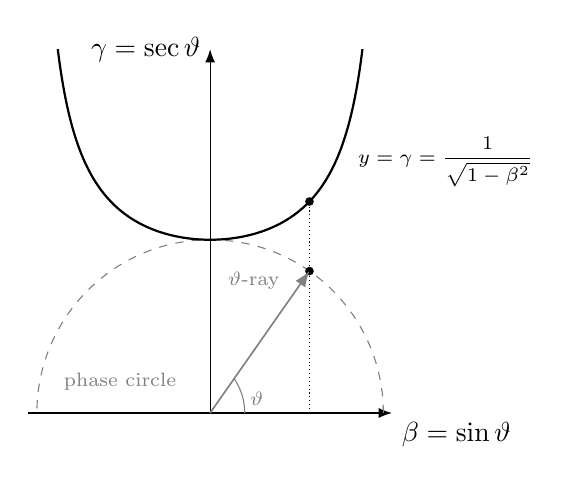
\begin{tikzpicture}[scale=2.2, >=Latex]
  % общие параметры
  \def\ymax{2.1}
  \def\th{35} % пример угла
  \pgfmathsetmacro{\bet}{sin(\th)}   % β = sin θ
  \pgfmathsetmacro{\co}{cos(\th)}    % cos θ
  \pgfmathsetmacro{\ga}{1/\co}       % γ = sec θ

  % оси (вне clip, чтобы надписи не резались)
  \draw[->] (-1.05,0) -- (1.05,0) node[below right] {$\beta=\sin\vartheta$};
  \draw[->] (0,0) -- (0,\ymax) node[left] {$\gamma=\sec\vartheta$};

  \begin{scope}
    \clip (-1.05,0) rectangle (1.95,\ymax);

    \draw[gray,dashed] (0,0) circle (1);

    \draw[line width=0.8pt] plot[domain=-0.90:0.90, samples=240] (\x, {1/sqrt(1-\x*\x)});

    \draw[densely dotted] (\bet,0) -- (\bet,\ga);
    \fill (\bet,\co) circle (0.025);
    \fill (\bet,\ga) circle (0.025);
  \end{scope}

  \draw[gray,->,line width=0.6pt] (0,0) -- (\bet,\co) node[pos=0.8, above left] {\scriptsize $\vartheta$-ray};
  \draw[gray] (0.20,0) arc[start angle=0, end angle=\th, radius=\th/100];
  \node[gray] at (0.27,0.08) {\scriptsize $\vartheta$};

  \node[gray] at (-0.52,0.18) {\scriptsize phase circle};
  \node at (1.36,1.45) {\scriptsize $y=\gamma=\dfrac{1}{\sqrt{1-\beta^{2}}}$};
\end{tikzpicture}
\caption{Phase circle vs. Lorentz hyperbola at common $\beta=\sin\vartheta$. Vertical mapping at fixed $\beta$ illustrates the Gudermann bridge: $\gamma=\sec\vartheta=\cosh\eta$.}
\label{fig:circle-hyperbola-gd}
\end{figure}
\FloatBarrier

%5 ===================================================================

\section{Phase space}

We represent a flow state on a quaternionic \emph{complex slice}
$\mathbb C_{\mathbf u}:=\mathrm{Span}\{1,\mathbf u\}\subset\mathbb H$,
where $\mathbf u\in S^2$ is the unit spatial direction selected by the observer’s split.
The unit rotor on this slice is
\[
\widehat q(\vartheta,\mathbf u):=\cos\vartheta+\mathbf u\,\sin\vartheta\in S^3\simeq SU(2),
\]
and, under the calibration $\|\boldsymbol\chi\|\equiv \clight$ (cf.\ §\ref{sec:calibration-c}),
we parameterize the flow vector as
\begin{equation}
\boldsymbol\chi(\vartheta,\mathbf u)=\clight\,\widehat q(\vartheta,\mathbf u)
=\clight\bigl(\cos\vartheta+\mathbf u\,\sin\vartheta\bigr).
\label{eq:phase-rotor-chi}
\end{equation}

\paragraph{Phase-rate projections (observer $A$).}\label{sec:phase-rates}
Given an observer $A$ with split $(\mathbf e_t^A,S^A)$ and
observer–object angle $\vartheta_{|\!A}$ (see \S\ref{sec:minkowski-derivation}),
the phase-rate components with respect to $A$ are
\begin{equation}
\tilde X^0_{|\!A}:=\frac{dx^0_{|\!A}}{d\chi}
=\clight\,\cos\vartheta_{|\!A},\qquad
\tilde{\mathbf X}_{|\!A}:=\frac{d\mathbf x_{|\!A}}{d\chi}
=\clight\,\sin\vartheta_{|\!A}\,\mathbf u_{|\!A},
\label{eq:phase-rates}
\end{equation}
where $\mathbf u_{|\!A}:=P_{S^A}\widehat{\mathbf F}/\|P_{S^A}\widehat{\mathbf F}\|\in S^A$ is the unit spatial
direction as seen by $A$ and $\widehat{\mathbf F}:=\boldsymbol\chi/\|\boldsymbol\chi\|$.

These rates satisfy the identity
\begin{equation}
\Bigl(\frac{ds}{d\chi}\Bigr)^2
=\bigl(\tilde X^0_{|\!A}\bigr)^2-\bigl\|\tilde{\mathbf X}_{|\!A}\bigr\|^2
=\clight^2\bigl(1-\sin^2\vartheta_{|\!A}\bigr)
=\clight^2\cos^2\vartheta_{|\!A}.
\label{eq:phase-budget-identity}
\end{equation}
which, in the SR simplification ($\zeta=\phi=0$ and $dt_A:=d\chi$), is just the operational split
of the fixed budget $\clight$ into temporal/spatial projections.

\paragraph{Phase-to-observable map (integral form).}
For any chart $x^i$ adapted to $A$ we have the integral transform
\begin{equation}
x^i(\chi)=x^i(\chi_0)+\int_{\chi_0}^{\chi}\tilde X^i_{|\!A}(u)\,du,
\qquad i=0,1,2,3,
\label{eq:phase-integral-map}
\end{equation}
with $\tilde X^0_{|\!A}$ and $\tilde{\mathbf X}_{|\!A}$ from \eqref{eq:phase-rates}. In the SR sector
this becomes
\(
t_A(\chi)=t_A(\chi_0)+\int_{\chi_0}^{\chi} du
\)
and
\(
\mathbf x_{|\!A}(\chi)=\mathbf x_{|\!A}(\chi_0)
+\int_{\chi_0}^{\chi}\clight\,\sin\vartheta_{|\!A}(u)\,\mathbf u_{|\!A}(u)\,du.
\)

\paragraph{Intrinsic vs.\ directional factors.}
The intrinsic second-moment angle $\zeta$ (\S\ref{sec:intrinsic-angle}) enters the body’s own
rate via $d\tau_B/d\chi=\cos\zeta$, while \eqref{eq:phase-rates} is purely directional and built
from the observer’s split. Outside the SR sector the intrinsic interval is
$ds_B^2=\clight^2\cos^2\zeta\,d\chi^2-d\boldsymbol\ell^{\!\top}\mathbf C_B\,d\boldsymbol\ell$,
and \eqref{eq:phase-integral-map} remains valid as a kinematic reconstruction of observables from
phase rates.

%6 ===================================================================
\section{Objects: operational catalogue and inference}
\label{sec:objects-catalogue}

\paragraph{Scope.} This section is a look-up summary. The physics and proofs live in
\S\ref{sec:body}, \S\ref{sec:intrinsic-angle}, \S\ref{sec:calibration-c}, and \S\ref{sec:phase-deriv}.

\subsection*{Canonical cases}
\begin{enumerate}
\item \textbf{Photon (vacuum).} \(\,T_B=0,\ d\tau_B=0,\ \|d\boldsymbol\ell\|/d\chi=\clight\) (Def.~\eqref{eq:calib-null}).
\item \textbf{Massive isotropic body.} \(\,\mathbf C_B=\frac{\sin^2\zeta}{3}\mathbf I,\quad
d\tau_B=\cos\zeta\,d\chi,\quad ds_B^2=\clight^2\cos^2\zeta\,d\chi^2-\frac{\sin^2\zeta}{3}\|d\boldsymbol\ell\|^2.\)
\item \textbf{Anisotropic body.} \(\,\mathbf C_B=\sum_{i=1}^3 \lambda_i\,\hat{\mathbf e}_i\otimes\hat{\mathbf e}_i,\ 
\lambda_i\ge0,\ \sum_i\lambda_i=\sin^2\zeta.\) Pullbacks along \(\hat{\mathbf e}_i\) probe \(\lambda_i\).
\item \textbf{Effective medium (\(\zeta\) only).} \(\,d\tau/dt=\cos\zeta,\ n(\zeta)=\sec\zeta\) (cf.\ \S\ref{ch:optics}).
\end{enumerate}

\subsection*{Parameter inference}
\begin{itemize}
\item \emph{Rate split at rest.} With \(\vartheta=0,\ \phi=0\): \(\cos\zeta=\bigl(d\tau_B/dt\bigr)_{\text{meas}}\).
\item \emph{Directional pullbacks.} Measure \(ds_B^2\) for small \(d\boldsymbol\ell\) along several lab directions;
fit the quadratic form \(q_B=d\boldsymbol\ell^\top\mathbf C_B\,d\boldsymbol\ell\Rightarrow\) eigenpairs \((\lambda_i,\hat{\mathbf e}_i)\).
\item \emph{Factorization with gravity/kinematics.} Use \(d\tau/dt=\cos\zeta\cos\phi\cos\vartheta\) to separate
\(\phi\) (clock angle) from \(\zeta\) via e.g.\ static vs moving protocols (see \S\ref{ch:optics}).
\end{itemize}

\subsection*{Ensemble composition}
For streamlets \(a\) with weights \(w_a\): \(T_B=\sum_a w_a\cos^2\Theta_a,\ 
\mathbf C_B=\sum_a w_a\sin^2\Theta_a\,\mathbf u_a\otimes\mathbf u_a\) (Eq.\ \eqref{eq:TB-CB}).

\subsection*{Non-collinear boosts}
Composition induces a spatial Wigner rotation on orientations without altering the scalar rate factorization;
see \S\ref{subsec:wigner}, \S\ref{subsec:thomas}.


%7 ===================================================================

\section{\texorpdfstring{Phase-derivative view}{Phase-derivative view}}
\label{sec:phase-deriv}

\noindent\textit{Scope.} This section repackages core identities in the language of
\emph{phase derivatives}, using only notions already introduced
(\S\ref{sec:calibration-c}–\ref{sec:minkowski-derivation}). No new kinematics is postulated.

\paragraph{Notation recap (from \S\ref{sec:phase-rates}).}
Phase–rate components for an observer $A$ are
\begin{equation}
\tilde X^0_{|\!A}=\frac{dx^0_{|\!A}}{d\chi}=\clight\,\cos\vartheta_{|\!A},\qquad
\tilde{\mathbf X}_{|\!A}=\frac{d\mathbf x_{|\!A}}{d\chi}
=\clight\,\sin\vartheta_{|\!A}\,\mathbf u_{|\!A},
\tag{\ref{eq:phase-rates}}
\end{equation}
and obey the identity
\begin{equation}
\Bigl(\frac{ds}{d\chi}\Bigr)^2
=\bigl(\tilde X^0_{|\!A}\bigr)^2-\bigl\|\tilde{\mathbf X}_{|\!A}\bigr\|^2
=\clight^2\bigl(1-\sin^2\vartheta_{|\!A}\bigr)
=\clight^2\cos^2\vartheta_{|\!A}.
\tag{\ref{eq:phase-budget-identity}}
\end{equation}
A change of parameter $\chi\mapsto\tau$ acts by the Jacobian $\mathcal J:=\dfrac{d\chi}{d\tau}$:
\begin{equation}
\dot X^i=\frac{d x^i}{d\tau}=\mathcal J\,\tilde X^i,\qquad
\dot{X}\equiv d/d\tau,\quad \tilde{X}\equiv d/d\chi.
\label{eq:param-change}
\end{equation}

\subsection{Minkowski–phase equality of invariants}
\label{subsec:phase-minkowski-equality}

\textbf{Theorem.} For any worldline segment and any observer $A$,
\begin{equation}
\boxed{\ \tilde H \;=\; \dot S\ },\qquad
\tilde H^2:=\bigl(\tilde X^0_{|\!A}\bigr)^2+\bigl\|\tilde{\mathbf X}_{|\!A}\bigr\|^2,\quad
\dot S^2:=\bigl(\dot X^0_{|\!A}\bigr)^2-\bigl\|\dot{\mathbf X}_{|\!A}\bigr\|^2 .
\label{eq:phase-minkowski-equality}
\end{equation}

\emph{Proof.} By \eqref{eq:param-change},
$\dot X^i=\mathcal J\,\tilde X^i$, hence
\[
\dot S^2=(\mathcal J\tilde X^0)^2-\|\mathcal J\tilde{\mathbf X}\|^2
=\mathcal J^2\!\left(\tilde X^0{}^2-\|\tilde{\mathbf X}\|^2\right)
=\mathcal J^2\Bigl(\frac{ds}{d\chi}\Bigr)^2
=\Bigl(\frac{ds}{d\tau}\Bigr)^2.
\]
At the same time,
$\tilde H^2=\tilde X^0{}^2+\|\tilde{\mathbf X}\|^2
=\clight^2$ in the SR gauge (\S\ref{subsec-1-5-sr-simplification}),
and $ds/d\tau=\clight$ by the operational split
$\cos\vartheta=d\tau/dt$, $\sin\vartheta=\|\mathbf v\|/\clight$ (\S\ref{sec:operational-phase}).
Therefore $\tilde H=\dot S=\clight$. $\square$

\paragraph{Reading.} In words: the Euclidean norm of the phase–rate vector equals the Minkowski
norm of the observable rate vector. The equality \eqref{eq:phase-minkowski-equality} is the
derivative form of “the same budget seen in two parametrizations”.

\subsection{Photon time: null interval and phase parameter}
\label{subsec:photon-phase-time}

For a lightlike flow in vacuum, the body’s intrinsic quadratic form gives
$ds_B^2=0$ (\S\ref{sec:calibration-c}), hence the body-level proper increment vanishes:
\begin{equation}
\boxed{\ d\tau_B=0\quad\text{(null flow, vacuum)}\ }.
\label{eq:photon-null}
\end{equation}
Nevertheless the phase parameter $\chi$ advances and serves as an affine parameter along
the ray. With the calibration \eqref{eq:calib-null} we have
\begin{equation}
\frac{\|d\boldsymbol\ell\|}{d\chi}=\clight,\qquad
\Rightarrow\quad \chi=\text{(cycle counter)}.
\label{eq:photon-affine}
\end{equation}

Under the convention $\Phi=\omega\,\chi$, one cycle corresponds to $\Delta\chi=2\pi/\omega$, so $\chi$ counts
wavefronts affinely while the intrinsic metric remains null ($d\tau_B=0$).


At unit frequency, $\nu:=d\chi/d\tau=1$, the phase equals the proper-time parameter used as an
affine label of wavefronts; no contradiction with \eqref{eq:photon-null} arises because
$\tau$ here is a \emph{chosen} parameter for counting cycles, while the intrinsic
metric length remains null.

% --- PATCH: insert after § Mapping to SR (before or after the correspondences table) ---

\subsection{Relativistic Doppler as a phase–kinematic theorem}\label{sec:doppler-core}

We derive the Doppler law purely from the phase split, without hyperbolic parametrization or dynamics.

\paragraph{Setup.}
Define frequency as the phase growth rate in proper time,
\(
\nu:=d\chi/d\tau
\),
and consider two successive wavefronts separated by the same phase increment
\(
\Delta\chi
\)
for the source and the observer. Then
\begin{equation}
\frac{\nu_{\mathrm{obs}}}{\nu_{\mathrm{src}}}
=\frac{d\chi/d\tau_{\mathrm{obs}}}{d\chi/d\tau_{\mathrm{src}}}
=\frac{d\tau_{\mathrm{src}}}{d\tau_{\mathrm{obs}}}.
\label{eq:doppler-core-master}
\end{equation}

In the SR sector (\(\zeta=\phi=0\)) the observer at rest has \(d\tau_{\mathrm{obs}}=dt_{\mathrm{obs}}\),
and for the (possibly moving) source \(dt_{\mathrm{src}}=\gamma\,d\tau_{\mathrm{src}}\) with
\(\gamma=\sec\vartheta\), \(\beta=\sin\vartheta\).

\paragraph{Longitudinal case.}
During the emission interval \(dt_{\mathrm{src}}=\gamma\,d\tau_{\mathrm{src}}\) (measured in the
observer’s lab chart) the source shifts by \(\pm \beta c\,dt_{\mathrm{src}}\) along the line of sight
(“\(+\)” receding, “\(-\)” approaching). The reception interval is the emission interval plus the
change in light flight time:
\[
dt_{\mathrm{obs}}
= dt_{\mathrm{src}} \,\bigl(1\pm \beta\bigr)
= \gamma\,d\tau_{\mathrm{src}} \,\bigl(1\pm \beta\bigr).
\]
With \eqref{eq:doppler-core-master} and \(d\tau_{\mathrm{obs}}=dt_{\mathrm{obs}}\) this gives the Doppler factor
\begin{equation}
\boxed{\ \frac{\nu_{\mathrm{obs}}}{\nu_{\mathrm{src}}}
=\frac{1}{\gamma(1\pm\beta)}\ }
=\sqrt{\frac{1\mp\beta}{1\pm\beta}}
=\sec\vartheta\,(1\mp\sin\vartheta)
=e^{\mp\eta},
\label{eq:doppler-core-long}
\end{equation}
where the equivalent forms use \(\beta=\sin\vartheta\), \(\gamma=\sec\vartheta\), and the Gudermann bridge \eqref{eq:gudermann}.

\paragraph{Transverse case.}
For \(\varphi=90^\circ\) (emission orthogonal to the relative velocity in the observer’s frame),
the geometric flight-time correction vanishes, hence
\begin{equation}
\boxed{\ \frac{\nu_{\mathrm{obs}}}{\nu_{\mathrm{src}}}=\frac{1}{\gamma}=\cos\vartheta\ }.
\label{eq:doppler-core-trans}
\end{equation}

\paragraph{General line-of-sight angle.}
Let \(\varphi\) be the angle between the source velocity and the line of sight in the observer’s frame.
Only the LOS component \(\beta\cos\varphi\) changes the flight time; repeating the above,
\begin{equation}
\boxed{\ \frac{\nu_{\mathrm{obs}}}{\nu_{\mathrm{src}}}
=\frac{1}{\gamma\,(1-\beta\cos\varphi)}
\ =\ \gamma\,(1-\beta\cos\varphi)^{-1}\ }.
\label{eq:doppler-core-los}
\end{equation}
Equivalently, in phase variables,
\(\nu_{\mathrm{obs}}/\nu_{\mathrm{src}}=\sec\vartheta\,\bigl(1-\sin\vartheta\cos\varphi\bigr)^{-1}\).

\paragraph{Corollary (with intrinsic/gravitational tilts).}
Outside the pure SR sector, the total redshift factorizes:
\[
1+z_{\rm tot}
=\frac{\nu_{\mathrm{src}}}{\nu_{\mathrm{obs}}}
=\underbrace{\gamma(1-\beta\cos\varphi)}_{\text{kinematic}}
\,\times\,
\underbrace{\frac{\cos\zeta_{\rm obs}\cos\phi_{\rm obs}}{\cos\zeta_{\rm src}\cos\phi_{\rm src}}}_{\text{intrinsic \& gravitational}},
\]
which reproduces \eqref{eq:z-factorization} upon identifying the kinematic part with
\eqref{eq:doppler-core-los}.

\paragraph{Infinitesimal form (longitudinal).}
Taking the differential of $\ln(\nu_{\mathrm{obs}}/\nu_{\mathrm{src}})$,
\begin{equation}
\boxed{\ d\ln\frac{\nu_{\mathrm{obs}}}{\nu_{\mathrm{src}}}
= \mp\,d\eta
= \mp\,\sec\vartheta\,d\vartheta
= \mp\,\gamma^{2}\,d\beta\ },
\label{eq:doppler-inf-long}
\end{equation}
with the upper sign for receding (“$+$” in \eqref{eq:doppler-core-long}) and lower for approaching.
Equation \eqref{eq:doppler-inf-long} is the \emph{phase–derivative} Doppler law.

\paragraph{Transverse case.}
For $\varphi=90^\circ$ in the observer’s frame the flight-time correction vanishes,
so $\nu_{\mathrm{obs}}/\nu_{\mathrm{src}}=1/\gamma$ and
\begin{equation}
d\ln\frac{\nu_{\mathrm{obs}}}{\nu_{\mathrm{src}}}=-\,d\ln\gamma=-\beta\gamma^2\,d\beta.
\label{eq:doppler-inf-trans}
\end{equation}

\paragraph{General LOS angle (fixed geometry).}
If $\varphi$ is the angle between the velocity and the line of sight in the observer’s frame and
$d\varphi=0$, then from
$\nu_{\mathrm{obs}}/\nu_{\mathrm{src}}=1/\bigl[\gamma(1-\beta\cos\varphi)\bigr]$ one gets
\begin{equation}
d\ln\frac{\nu_{\mathrm{obs}}}{\nu_{\mathrm{src}}}
=-\Bigl[\beta\gamma^2-\frac{\cos\varphi}{1-\beta\cos\varphi}\Bigr]\,d\beta
\ =\ -\,d\eta\ \ \text{when }\ \varphi=0,\pi .
\label{eq:doppler-inf-los}
\end{equation}

\medskip
Together, \eqref{eq:phase-minkowski-equality}, \eqref{eq:photon-null}–\eqref{eq:photon-affine}, and
\eqref{eq:doppler-inf-long}–\eqref{eq:doppler-inf-los} show how \emph{phase derivatives} encode:
(i) equality of observable and phase invariants;
(ii) the null nature of photon proper time with $\chi$ as an affine counter;
(iii) the Doppler law, both finite and in instantaneous differential form.

%8 ===================================================================

\section{Unified temporal effects in phase space}
\label{ch:optics}

We factor all time-related effects through a single phase tilt structure.
Let the intrinsic (\(\zeta\)), gravitational (\(\phi\)), and kinematic (\(\vartheta\)) angles be independent contributors to the phase tilt at a point.
Define the local \emph{time-rate factor}
\begin{equation}
\label{eq:time-rate-factor}
\frac{d\tau}{dt}
\;=\;
\cos\zeta\;\cos\phi\;\cos\vartheta,
\qquad
n_{\rm tot}\;:=\;\sec\zeta\;\sec\phi\;\sec\vartheta,
\end{equation}
where \(n_{\rm tot}\) plays the role of an effective (phase) refractive index for light propagation.
Accordingly, the coordinate light-travel time along a spatial curve \(\Gamma\) is
\begin{equation}
\label{eq:optical-length}
t_\Gamma \;=\; \frac{1}{\clight}\int_\Gamma n_{\rm tot}\,ds.
\end{equation}

\paragraph{Lemma (Unified time-rate).}
In the unimetry phase representation, the proper-to-lab time rate and the optical length factorize as in \eqref{eq:time-rate-factor}–\eqref{eq:optical-length}.
Setting any subset of angles to zero recovers the corresponding standard effects:
\begin{itemize}\itemsep4pt
  \item \textbf{Special relativity (vacuum SR):} \(\zeta=0,\ \phi=0\Rightarrow d\tau/dt=\cos\vartheta=1/\gamma\) (kinematic time dilation).
  \item \textbf{Gravitational clocks (static weak field):} \(\zeta=0,\ \vartheta=0\Rightarrow d\tau/dt=\cos\phi\) (gravitational redshift/clock rate); calibration of \(\phi\) reproduces the usual \(\sqrt{g_{00}}\).
  \item \textbf{Shapiro delay (gravitational contribution to TOF):} with \(\zeta=0,\ \vartheta=0\), \eqref{eq:optical-length} yields \(t_\Gamma=(1/\clight)\int \sec\phi\,ds\); the excess over \(\int ds/\clight\) is the Shapiro time delay.
  \item \textbf{Intrinsic/evolutionary tilt:} \(\phi=0,\ \vartheta=0\Rightarrow d\tau/dt=\cos\zeta,\ n_{\rm tot}=\sec\zeta\) (useful as a time gauge in cosmological/effective-medium contexts).
\end{itemize}

\paragraph{Remarks.}
(i) The factorization in \eqref{eq:time-rate-factor} is the phase-space counterpart of composing independent tilts; it preserves the conserved Minkowski norm once time is reparameterized by \(\tau\).
(ii) For vacuum SR we simply set \(\zeta=0\) and work with \(\vartheta\); for pure gravitational timing we set \(\vartheta=0\) and use \(\phi\).
(iii) Non-collinear boost composition acts on \(\vartheta\) via quaternionic rotors and induces a Wigner/Thomas residual \emph{spatial} rotation without altering \eqref{eq:time-rate-factor}.

%9 ===================================================================

\section{\texorpdfstring{Gravity as a phase rotation: local tetrads and clock angle}{Gravity as a phase rotation}}

On a curved background $(\mathcal M,g)$ we work with orthonormal tetrads $e_a{}^\mu$ such that $g_{\mu\nu}e_a{}^\mu e_b{}^\nu=\eta_{ab}$ and take the observer's time leg to be $e_0{}^\mu$. 
We apply the gravitational (clock) angle $\phi$ as
\begin{equation}
\cos\phi\ :=\ e^0{}_\mu\,u^\mu\ =\ \frac{d\tau_{\rm stat}}{dt}\ =\ \sqrt{-g_{00}}\qquad\text{(stationary case)}.
\label{eq:clock-angle}
\end{equation}

Kinematics remains encoded by the phase angle $\vartheta$ in the slice $\mathbb C_{\mathbf u}$, with
$\cos\vartheta=d\tau/d\tau_{\rm stat}$. 
Therefore the proper time factorizes as
\begin{equation}
d\tau\ =\ dt\,\cos\phi\,\cos\vartheta,\qquad 
d\mathbf x\ =\ c\,dt\,\sin\vartheta\,\mathbf u,
\label{eq:tau-factorization}
\end{equation}
and the total redshift factorizes into kinematic and gravitational parts:
\begin{equation}
1+z_{\rm tot}\ =\ \frac{\cos\vartheta_{\rm em}}{\cos\vartheta_{\rm obs}}\ \times\ 
\frac{\cos\phi(x_{\rm em})}{\cos\phi(x_{\rm obs})}.
\label{eq:z-factorization}
\end{equation}

For static emitter/observer ($\vartheta_{\rm em}=\vartheta_{\rm obs}=0$) one recovers the standard gravitational redshift 
$1+z_g=\sqrt{\frac{-g_{00}(x_{\rm obs})}{-g_{00}(x_{\rm em})}}$.
In the weak-field limit $g_{00}\simeq-(1+2\Phi/ \clight^2)$ this gives $z_g\simeq(\Phi_{\rm obs}-\Phi_{\rm em})/c^2$.

\paragraph{Beyond static fields.}
In a $3\!+\!1$ split $ds^2=-N^2 \clight^2 dt^2 + h_{ij}(dx^i+N^i dt)(dx^j+N^j dt)$ one may identify $\cos\phi:=N$ in the observer's tetrad, which keeps \eqref{eq:tau-factorization}–\eqref{eq:z-factorization} coordinate-agnostic.
Uniform acceleration (Rindler) accumulates phase according to $d\vartheta=\kappa\,dt$ inside the local slice, consistently reproducing accelerated-frame kinematics when combined with the clock angle $\phi$.

%9 ===================================================================

\section{Discussion}

The phase-space reformulation of special relativity presented in this work provides an original and conceptually unifying framework, recasting all standard kinematic effects as geometric projections and rotations within a Euclidean (as opposed to pseudo-Euclidean) phase space structured by the algebra of quaternions. This approach enables closed-form derivations of time dilation, Lorentz contraction, all Doppler effects, and the composition of boosts—including the emergence of Wigner and Thomas rotations—as pure consequences of phase kinematics and composition rules for rotors. Notably, the speed of light appears not as a postulate but as a derived invariant: the magnitude of the calibrated flow.

One of the main strengths of the unimetry approach is its ability to coherently and transparently separate intrinsic, gravitational, and kinematic effects through the introduction of independent angular parameters. This structural modularity allows for clear generalizations beyond the regime of special relativity (SR). The use of quaternionic algebra naturally incorporates the noncommutative composition of boosts (and hence Wigner rotation), and the direct operational mapping from phase parameters to observable quantities avoids the hyperbolic constructs and nested root expressions traditional to the Lorentzian metric, potentially offering both conceptual and computational simplifications.

The revisit of the kinematical foundations of relativity within a Euclidean metric is reminiscent of various efforts to find deeper group-theoretic or geometric underpinnings for known physics, such as the reinterpretation of quantum spinors, twistors, or the generalized use of Clifford and quaternionic structures. 

Despite these advantages, there are several limitations and open issues:
\begin{itemize}
    \item The present work, while offering a full reformulation of SR, leaves the dynamical aspects---especially those tied to gravitational fields and interactions---outside its direct scope. The approach to gravity as a phase tilt field is promising, but it will require a precise translation of Einsteinian field dynamics into the quaternionic, phase-based language.
    \item Similarly, the connection to quantum mechanics, though structurally motivated by the phase-space formulation and inherent links to phase and geometric quantization, remains undeveloped at the level of operator theory or Hilbert space structures. Concrete examples or models connecting unimetry directly to quantum phenomena would reinforce the physical scope and relevance of the approach.
    \item A key question for future study is the physical interpretability and experimental accessibility of the various angular parameters (intrinsic, gravitational, kinematic) in more complex, curved, or quantum-influenced scenarios.
    \item The mathematical tools used---particularly the phase decomposition and modularization---have strong implications for the construction of algorithms in numerical relativity and simulation of accelerated particle beams, but explicit comparisons with existing computational methods remain to be presented.
\end{itemize}


\section*{Outlook}

The unimetry framework developed here provides a versatile foundation for future theoretical developments in both relativity and quantum physics. The following directions emerge as particularly promising:
\begin{itemize}
    \item
    \textbf{Extension to General Relativity.} The modular phase decomposition is well suited for the introduction of curved metrics, potentially allowing gravitational redshift, time delay (Shapiro effect), and even curvature-driven precessions to be recast in the language of phase tilts and generalized rotors. Realizing Einstein's dynamics for gravitational fields in this formalism is a natural next step, especially via the local tetrad and clock angle structures already sketched.

    \item
    \textbf{Quantum Connections.} Given the central role of phase, rotors, and symmetry groups (notably the demonstration of Hopf fibration structure), the unimetry formalism can serve as a stepping stone toward a deeper unification between relativistic and quantum frameworks, possibly via geometric quantization or generalized qubit/Bloch-sphere analogues.

    \item
    \textbf{Physical and Experimental Applications.} The structure is already suited for reinterpretation and numerical simulation of phenomena involving non-collinear accelerations, such as in advanced particle beam physics or optical systems with phase media. This computational potential deserves further methodological and comparative exploration.

    \item
    \textbf{Generalizations and Group Theory.} The embedding of Lorentzian kinematics within a more general Euclidean group-theoretic framework (potentially encompassing de Sitter or conformal transformations) may suggest further extensions, including nontrivial topologies, higher dimensions, or self-dual (instanton-like) solutions.
\end{itemize}

In summary, by replacing the traditional spacetime paradigm with a geometric flow in phase space, unimetry opens avenues for new mathematical structures and connections among relativity, geometry, and quantum theory. Its broader success will depend on future progress in developing the gravitational and quantum sectors and on the demonstration of concrete computational and experimental advantages.




\appendix
\section{Equivalence to the classical Wigner rotation}
\label{app:1}

We sketch an intrinsic quaternionic proof that the unimetry expression for the Wigner rotation
coincides with the standard special-relativistic formula.

\paragraph{Step 1: product of two D-rotors.}
For $d_i=\cos\frac{\psi_i}{2}+\uhat_i\sin\frac{\psi_i}{2}$,
\begin{equation}
\label{eq:auto:45}
d_2 d_1
=(c_2c_1-s_2s_1\cos\theta)
+\Big(c_2s_1\uhat_1+s_2c_1\uhat_2+s_2s_1\,\uhat_2\times\uhat_1\Big),
\end{equation}
with $c_i=\cos(\psi_i/2)$, $s_i=\sin(\psi_i/2)$ and $\cos\theta=\uhat_2\!\cdot\!\uhat_1$.

\paragraph{Step 2: symmetric D--R factorization.}
Define $d_{12}$ by $d_{12}\,\mathbf e_t\, d_{12}=L_{12}\,\mathbf e_t\, L_{21}$ and set
$r_W=\bar d_{12}\,L_{12}=L_{21}\,\bar d_{12}$. Then $r_W$ fixes $\mathbf e_t$ and is a pure spatial
rotor, so $r_W=\cos\frac{\phi}{2}+\hat{\mathbf n}\sin\frac{\phi}{2}$ with
$\hat{\mathbf n}\parallel \uhat_2\times\uhat_1$. Matching scalar and bivector parts gives
\begin{equation}
\tan\frac{\phi}{2}=
\frac{s_1 s_2\,\sin\theta}{\,c_1 c_2+s_1 s_2\,\cos\theta\,}.
\label{eq:uni-phi}
\end{equation}

\paragraph{Step 3: map to rapidities.}
With the substitutions $\sin(\psi/2)\mapsto\sinh(\eta/2)$, $\cos(\psi/2)\mapsto\cosh(\eta/2)$,
$\tan(\psi/2)\mapsto\tanh(\eta/2)$ (where $\tanh\eta=\beta$, $\cosh\eta=\gamma$), \eqref{eq:uni-phi}
becomes the textbook Wigner angle:
\begin{equation}
\label{eq:auto:47}
\tan\frac{\phi}{2}
=\frac{\sinh\frac{\eta_1}{2}\,\sinh\frac{\eta_2}{2}\,\sin\theta}
{\cosh\frac{\eta_1}{2}\,\cosh\frac{\eta_2}{2}+\sinh\frac{\eta_1}{2}\,\sinh\frac{\eta_2}{2}\,\cos\theta},
\end{equation}
with axis along $\uhat_2\times\uhat_1$. This circular--hyperbolic correspondence is classical; cf.\ Gudermann~\cite{Gudermann1830}.

\end{document}
